% !TeX program = lualatex

\documentclass[oneside]{academica}
\usepackage{booktabs}
\usepackage{stmaryrd} % for llbracket
\usepackage{enumitem}
\usepackage{adjustbox} % for too wide tikz

\usetikzlibrary{arrows,angles,quotes,quantikz2}
\tikzset{phase/.append style={scale=2}}

%   \lstset{basicstyle=\ttfamily\small, breaklines=true,
%           keywordstyle=\color{blue!70!black},
%           commentstyle=\color{green!50!black},
%           stringstyle=\color{red!60!black},
%           frame=single, rulecolor=\color{gray!40},
%           backgroundcolor=\color{gray!5},
%           numbers=left, numberstyle=\tiny\color{gray}}

\setlength{\parindent}{0pt}

\DeclareMathOperator{\tr}{Tr}

\renewcommand{\H}{\mathcal{H}}


\overtitle{notes for}
\title{Quantum Computing \& Communication}
\author{Merlo Filippo}

\begin{document}

\frontmatter
\maketitle
\tableofcontents
\mainmatter

\chapter{Mathematical Foundations}

\section{Complex Numbers}

The real numbers are not algebraically closed: the equation $x^2+1=0$ has no real solution.
We extend $\mathbb{R}$ by adjoining a symbol $i$ defined to satisfy $i^2 = -1$, obtaining the \textbf{complex numbers} $\mathbb{C}$.

\begin{definition*}[Complex number]
  A \emph{complex number} is a pair $(a,b)\in\mathbb{R}^2$ written as $z = a + ib$, where $a = \operatorname{Re}(z)$ is the \emph{real part} and $b = \operatorname{Im}(z)$ is the \emph{imaginary part}.
\end{definition*}

The arithmetic rules follow from $i^2=-1$:
\begin{align*}
  (a+ib)+(c+id) &= (a+c)+i(b+d) \\
  (a+ib)(c+id)  &= (ac-bd)+i(bc+ad)
\end{align*}
The \textbf{complex conjugate} of $z=a+ib$ is $z^*=a-ib$ (negate the imaginary part).
Its most important property is
\begin{equation*}
  z\,z^* = a^2+b^2 \ge 0
\end{equation*}
which is always real and non-negative.
This lets us define the \textbf{modulus} $|z|=\sqrt{z\,z^*}=\sqrt{a^2+b^2}$, the distance from $z$ to the origin in the complex plane.

\subsection{Polar Form and Euler's Formula}

Every complex number can be written in \emph{polar form} using its modulus $r=|z|$ and its \emph{argument} (angle) $\theta$:
\begin{equation*}
  z = r\,e^{i\theta} = r(\cos\theta + i\sin\theta)
\end{equation*}
This is \textbf{Euler's formula}, one of the most useful identities in all the mathematics.
When $r=1$ the number lives on the \emph{unit circle} $|z|=1$, and multiplication by $e^{i\theta}$ is a rotation by angle $\theta$.

\begin{example*}[The four fourth roots of unity]
  The solutions of $z^4=1$ are $z=e^{2\pi i k/4}$ for $k=0,1,2,3$, giving $1,\,i,\,-1,\,-i$.
  Notice they lie equally spaced on the unit circle.
  This pattern generalizes: the $N$ solutions of $z^N=1$ are $\omega^k$ where $\omega=e^{2\pi i/N}$, and they are the backbone of the quantum Fourier transform.
\end{example*}

\section{Vector Spaces and Dirac Notation}

\begin{definition*}[Vector space]
  A \emph{vector space} over $\mathbb{C}$ is a set $V$ together with operations of addition and scalar multiplication satisfying the usual axioms (associativity, commutativity, distributivity, existence of zero, etc.).
\end{definition*}

The most important example for us is $\mathbb{C}^n$, the set of $n$-tuples of complex numbers.
Quantum states will live in $\mathbb{C}^2$ (for one qubit), $\mathbb{C}^4$ (for two qubits), and $\mathbb{C}^{2^n}$ in general.

Physicists write column vectors as \textbf{kets} $\ket{v}$ and row vectors as \textbf{bras} $\bra{v}$.
The pairing is:
\begin{equation*}
  \ket{v} = \begin{bmatrix}v_1\\\vdots\\v_n\end{bmatrix} \in \mathbb{C}^n, \qquad
  \bra{v} = \ket{v}^\dagger = \begin{bmatrix}v_1^*&\cdots&v_n^*\end{bmatrix}
\end{equation*}
where $\dagger$ denotes \emph{conjugate transpose} (transpose then conjugate each entry).
The \textbf{inner product} of two vectors is then the \emph{bra-ket} (hence ``braket'' notation):
\begin{equation*}
  \braket{u}{v} = \bra{u}\ket{v} = u_1^*v_1+\cdots+u_n^*v_n \;\in\;\mathbb{C}
\end{equation*}

Key properties of the inner product:
\begin{itemize}
  \item \textbf{Conjugate symmetry} (sesquilinearity): $\braket{u}{v}=\braket{v}{u}^*$; equivalently, the inner product is \emph{linear} in the second argument and \emph{antilinear} (conjugate-linear) in the first: $\bra{\lambda u+\mu v} = \lambda^*\bra{u}+\mu^*\bra{v}$.
  \item \textbf{Linearity in second argument}: $\braket{u}{\alpha v+\beta w}=\alpha\braket{u}{v}+\beta\braket{u}{w}$
  \item \textbf{Positive definiteness}: $\braket{v}{v}\ge 0$, with equality iff $\ket{v}=\mathbf{0}$
\end{itemize}

The \textbf{norm} of a vector is $\|\ket{v}\|=\sqrt{\braket{v}{v}}$.
Two vectors are \textbf{orthogonal} when $\braket{u}{v}=0$.
A set of vectors is \textbf{orthonormal} if they are pairwise orthogonal and each has norm 1.

The \textbf{outer product} $\ket{u}\bra{v}$ (ket times bra) is an $n\times n$ matrix:
\begin{equation*}
  \ket{u}\bra{v} = \begin{bmatrix}u_1\\\vdots\\u_n\end{bmatrix}
  \begin{bmatrix}v_1^*&\cdots&v_n^*\end{bmatrix}
\end{equation*}
This is not a number; it is a rank-1 linear operator.

\begin{definition*}[Linear combination]
  The \emph{linear combination} of a set of vectors $\{\ket{v_1},\ldots,\ket{v_n}\}$ is any sum of the form
  \begin{equation*}
    \sum_{i=1}^n a_i\ket{v_i}
  \end{equation*}
  with $a_i\in\mathbb{C}$.
\end{definition*}

A set of vectors is \textbf{linearly dependent} if at least one of them can be written as a linear combination of the others; otherwise it is \textbf{linearly independent}.

\begin{definition*}[Span]
  The \emph{span} of $S=\{v_1,\ldots,v_n\}$ is the set of all linear combinations:
  \begin{equation*}
    \text{span}(S)=\left\{\sum_i a_i v_i \mid a_i\in\mathbb{C}\right\}
  \end{equation*}
  If $\text{span}(S)=V$ then $S$ is a \emph{spanning set} for $V$.
\end{definition*}

The distinction between a spanning set and its span is worth emphasizing.
For example, $\{\ket{0},\ket{1}\}$ is a spanning set of just two vectors, while its span is $\{\alpha\ket{0}+\beta\ket{1}\mid\alpha,\beta\in\mathbb{C}\}$, \ie, the entire (infinite) space of qubit states.

A \textbf{basis} of $\mathbb{C}^n$ is a minimal spanning set: a set of $n$ linearly independent vectors such that every element of $\mathbb{C}^n$ is a \emph{unique} linear combination of them.

The most natural basis for quantum computing is the \textbf{computational basis}, whose elements are standard unit vectors:
\begin{equation*}
  \ket{0}=\begin{bmatrix}1\\0\end{bmatrix},\quad
  \ket{1}=\begin{bmatrix}0\\1\end{bmatrix},\quad
  \ket{00}=\begin{bmatrix}1\\0\\0\\0\end{bmatrix},\quad
  \ket{01}=\begin{bmatrix}0\\1\\0\\0\end{bmatrix},\quad\ldots
\end{equation*}
The $n$-qubit computational basis has $2^n$ elements, one for each binary string of length $n$.
Any quantum state can be written as a linear combination of them.
Another useful basis for a single qubit is the \textbf{Hadamard basis}:
\begin{equation*}
  \ket{+}=\frac{\ket{0}+\ket{1}}{\sqrt{2}},\qquad \ket{-}=\frac{\ket{0}-\ket{1}}{\sqrt{2}}
\end{equation*}
These are the $+1$ and $-1$ eigenstates of the Pauli $X$ gate, and will appear constantly in algorithms.

\begin{definition*}[Orthonormal basis]
  A basis $\{\ket{v_i}\}$ of an inner product space is \emph{orthonormal} if
  $\braket{v_i}{v_j}=\delta_{ij}$ for all $i,j$.
\end{definition*}

It is often useful to express the same operator or state in a different basis.
If $\{\ket{u_i}\}$ and $\{\ket{v_i}\}$ are two orthonormal bases, each basis vector can be written as a linear combination of the other:
\begin{equation*}
  \ket{v_i} = \sum_j R_{ij}\ket{u_j}
\end{equation*}
The \textbf{change-of-basis matrix} $R$ is always \emph{unitary} when both bases are orthonormal, so $R^{-1}=R^\dagger$ and $RR^\dagger=R^\dagger R=I$.
An operator $A$ expressed in basis $\{\ket{u_i}\}$ transforms to $R^\dagger AR$ in basis $\{\ket{v_i}\}$.

\begin{note}
  Unitary operators $\subseteq$ Normal operators $\supseteq$ Hermitian operators.
  Hermitian and unitary matrices are always normal, but unitary matrices are not generally Hermitian, and vice versa.
\end{note}

\section{Linear Operators and Matrices}

\begin{definition*}[Linear operator]
  A map $A:V\to V$ is \emph{linear} if $A(c_1\ket{v_1}+c_2\ket{v_2})=c_1 A\ket{v_1}+c_2 A\ket{v_2}$.
\end{definition*}

Once a basis is fixed, every linear operator on $\mathbb{C}^n$ is represented by an $n\times n$ complex matrix, and operator composition becomes matrix multiplication.
The entry $(A)_{ij}=\bra{i}A\ket{j}$ gives the matrix in any orthonormal basis $\{\ket{i}\}$.

\subsection{Adjoint, Hermitian, Unitary}

The \textbf{adjoint} (or \emph{conjugate transpose}) of $A$ is the matrix $A^\dagger$ satisfying $\braket{u}{Av}=\braket{A^\dagger u}{v}$
for all $\ket{u},\ket{v}$.
Concretely, $(A^\dagger)_{ij}=A_{ji}^*$.

Three special classes of operators arise everywhere in quantum theory:
\begin{center}
  \renewcommand{\arraystretch}{1.3}
  \begin{tabular}{l|l|l}
    \textbf{Name} & \textbf{Condition} & \textbf{Role in QC} \\
    \hline
    Hermitian (self-adjoint) & $A=A^\dagger$ & Observable quantities \\
    Unitary & $U U^\dagger = U^\dagger U = I$ & Quantum gates / time evolution \\
    Normal & $A A^\dagger = A^\dagger A$ & Includes both above \\
  \end{tabular}
\end{center}

Unitary operators preserve the inner product:
$\braket{U u}{U v}=\braket{u}{v}$, so they preserve norms and hence
probabilities.
This is why every valid quantum gate must be unitary.

\begin{example*}[Verifying the Hadamard gate is unitary]
  $H=\frac{1}{\sqrt{2}}\begin{bmatrix}1&1\\1&-1\end{bmatrix}$.
  Then $H^\dagger=H$ (it's also Hermitian!), and
  \begin{equation*}
    H^\dagger H = H^2 = \frac{1}{2}\begin{bmatrix}1&1\\1&-1\end{bmatrix}
    \begin{bmatrix}1&1\\1&-1\end{bmatrix}
    =\frac{1}{2}\begin{bmatrix}2&0\\0&2\end{bmatrix}=I.
  \end{equation*}
  Since $H^2=I$, applying $H$ twice returns the original state.
\end{example*}

\subsection{Eigenvalues}

For a linear operator $A$, a nonzero vector $\ket{v}$ is an
\textbf{eigenvector} with \textbf{eigenvalue} $\lambda$ when
$A\ket{v}=\lambda\ket{v}$.
Eigenvalues are found by solving
$\det(A-\lambda I)=0$, a degree-$n$ polynomial (so there are exactly
$n$ eigenvalues, counting multiplicity, in $\mathbb{C}$).

\begin{theorem}[Spectral decomposition]\label{th:spectral}
  Any normal operator $A$ on $\mathbb{C}^n$ can be written as
  \begin{equation*}
    A = \sum_{i=1}^n \lambda_i \ket{v_i}\bra{v_i}
  \end{equation*}
  where $\{\ket{v_i}\}$ is an orthonormal basis of eigenvectors and
  $\lambda_i$ are the corresponding eigenvalues.
Equivalently,
  $A=R D R^\dagger$ where $D$ is diagonal with the eigenvalues and
  $R$ is unitary with the eigenvectors as columns.
\end{theorem}

Important corollaries:
\begin{itemize}
  \item \textbf{Hermitian operators} have \emph{real} eigenvalues.
    (Proof: $\lambda=\bra{v}A\ket{v}=\bra{v}A^\dagger\ket{v}=\lambda^*$.)
    This is why observables are Hermitian: physical measurement
    outcomes must be real numbers.
  \item \textbf{Unitary operators} have eigenvalues on the unit circle,
    of the form $e^{i\phi}$.
(Proof: $|\lambda|^2=\lambda\lambda^*=\bra{v}U^\dagger U\ket{v}=1$.)
  \item \textbf{Normal operators} have orthogonal eigenvectors: if $\lambda_i\neq\lambda_j$ then $\braket{v_i}{v_j}=0$.
\end{itemize}

The \textbf{eigenvalue equation} for an $n\times n$ matrix $A$ is $\det(A-\lambda I)=0$, a degree-$n$ polynomial in $\lambda$ with exactly $n$ roots (counting multiplicity) in $\mathbb{C}$.
For each eigenvalue $\lambda_i$ one then solves $A\ket{v}=\lambda_i\ket{v}$ for the corresponding eigenvector.
The \textbf{rank} of a matrix is the maximum number of linearly independent columns (equivalently, rows); linear dependence of the columns of a square matrix implies linear dependence of its rows.

\subsection{Trace}

\begin{definition*}[Trace]
  The \emph{trace} of a matrix is the sum of its diagonal entries:
  $\tr(A)=\sum_i A_{ii}$.
\end{definition*}

The trace has three fundamental properties:
\begin{itemize}
  \item \textbf{Cyclic}: $\tr(ABC)=\tr(BCA)=\tr(CAB)$.
  \item \textbf{Linear}: $\tr(A+B)=\tr(A)+\tr(B)$, $\tr(zA)=z\tr(A)$.
  \item \textbf{Basis-independent}: $\tr(A)=\sum_i\lambda_i$ (equals the sum of eigenvalues, regardless of which basis is used to compute the diagonal).
\end{itemize}
It will appear everywhere when computing measurement probabilities.

\subsection{Projection}

A \textbf{projector} along the direction of a unit vector $\ket{u}$ is
\begin{equation*}
  P_u = \ket{u}\bra{u}
\end{equation*}
(for a normalized $\ket{u}$).
It projects any vector onto the direction of $\ket{u}$:
$P_u\ket{\psi} = \braket{u}{\psi}\ket{u}$.

Every projector satisfies $P^2=P$ (idempotence):
\begin{equation*}
  P_u^2 = (\ket{u}\bra{u})(\ket{u}\bra{u}) = \ket{u}\underbrace{\braket{u}{u}}_{1}\bra{u} = \ket{u}\bra{u} = P_u
\end{equation*}

Any state $\ket{\psi}$ can be decomposed into its component along $\ket{u}$ and the orthogonal remainder:
\begin{equation*}
  \ket{\psi} = \underbrace{P_u\ket{\psi}}_{\ket{\psi_u}} + \underbrace{(I-P_u)\ket{\psi}}_{\ket{\psi_{\perp u}}}
\end{equation*}

\subsection{Functions of Operators}

If $f(x)=\sum_k f_k x^k$ has a power series expansion, define
\begin{equation*}
  f(A) = \sum_k f_k A^k
\end{equation*}
Using the spectral decomposition $A=\sum_i\lambda_i\ket{v_i}\bra{v_i}$, one can show $A^n=\sum_i\lambda_i^n\ket{v_i}\bra{v_i}$, and therefore
\begin{equation*}
  f(A) = \sum_i f(\lambda_i)\ket{v_i}\bra{v_i}
\end{equation*}
This is extremely useful for computing things like $e^{iHt}$ (the time-evolution operator) and $\sqrt{A}$ (needed for polar decomposition).

\begin{example*}
  For the Pauli $Z$ gate with eigenvalues $\pm1$ and eigenvectors $\ket{0},\ket{1}$:
  \begin{equation*}
    e^{i\theta Z} = e^{i\theta}\ket{0}\bra{0} + e^{-i\theta}\ket{1}\bra{1}
    = \begin{bmatrix}e^{i\theta}&0\\0&e^{-i\theta}\end{bmatrix} = R_z(-2\theta)
  \end{equation*}
  (up to global phase).
This shows directly how the rotation gate $R_z$ arises from the Hamiltonian $H=Z$.
\end{example*}

\section{Tensor Products}

The tensor product is the mathematical operation that combines two
independent systems into one joint system.

\begin{definition*}[Tensor product of vector spaces]
  If $U$ is $m$-dimensional and $V$ is $n$-dimensional, their tensor
  product $U\otimes V$ is $mn$-dimensional.
Its elements are formal
  linear combinations of \emph{product vectors} $\ket{u}\otimes\ket{v}$
  (also written $\ket{u}\ket{v}$ or $\ket{uv}$).
\end{definition*}

Concretely, for column vectors:
\begin{equation*}
  \begin{bmatrix}u_1\\u_2\end{bmatrix}\otimes\begin{bmatrix}v_1\\v_2\end{bmatrix}
  =\begin{bmatrix}u_1 v_1\\u_1 v_2\\u_2 v_1\\u_2 v_2\end{bmatrix}
\end{equation*}

For operators (the \textbf{Kronecker product}):
\begin{equation*}
  A\otimes B = \begin{bmatrix}A_{11}B&\cdots&A_{1n}B\\\vdots&\ddots&\vdots\\A_{n1}B&\cdots&A_{nn}B\end{bmatrix}
\end{equation*}

\begin{example*}[$H\otimes H$ and the uniform superposition]
  \begin{equation*}
    H\otimes H =
    \frac{1}{2}\begin{bmatrix}1&1&1&1\\1&-1&1&-1\\1&1&-1&-1\\1&-1&-1&1\end{bmatrix}
  \end{equation*}
  Applying this to $\ket{00}$ gives
  $\frac{1}{2}(\ket{00}+\ket{01}+\ket{10}+\ket{11})$,
  the uniform superposition over all two-bit strings.
  This generalizes: $H^{\otimes n}\ket{0}^{\otimes n}=
  \frac{1}{\sqrt{2^n}}\sum_{x=0}^{2^n-1}\ket{x}$, which is the
  starting point of most quantum algorithms.
\end{example*}

\begin{example*}[Kronecker product of $\sigma_x$ and $\sigma_z$]
  \begin{align*}
    \sigma_x\otimes\sigma_z
    &= \begin{bmatrix}0\cdot\sigma_z & 1\cdot\sigma_z\\1\cdot\sigma_z & 0\cdot\sigma_z\end{bmatrix}
    = \begin{bmatrix}
        0 & 0 & 1 & 0\\
        0 & 0 & 0 & -1\\
        1 & 0 & 0 & 0\\
        0 & -1 & 0 & 0
      \end{bmatrix}
  \end{align*}
  where each $A_{ij}$ is replaced by $A_{ij}\cdot\sigma_z$.
  Notice how the block structure mirrors $\sigma_x$: the top-right and bottom-left blocks are $\sigma_z$, and the diagonal blocks are $0\cdot\sigma_z=0$.
\end{example*}


\begin{exercise*}[The SWAP-like operator $H=\tfrac{1}{2}(\sigma_x\otimes\sigma_x+\sigma_y\otimes\sigma_y+\sigma_z\otimes\sigma_z+I\otimes I)$]
  Let $H=\tfrac{1}{2}(\sigma_x\otimes\sigma_x+\sigma_y\otimes\sigma_y+\sigma_z\otimes\sigma_z+I\otimes I)$.
  \begin{enumerate}[label=\alph*)]
    \item Show that $H^2=I$ (\ie, $H$ is the SWAP operator).
    \item Write $e^{-iH\theta}$ in closed form.
    \item Find the eigenvalues of $H$.
  \end{enumerate}

  \textbf{Part a): $H^2=I$.}
  One can verify directly that $H$ is the SWAP operator
  (it exchanges the two qubits: $H\ket{xy}=\ket{yx}$), so $H^2=I$.
  Alternatively, use the Pauli identity $\sigma_i^2=I$ and
  $\sigma_i\sigma_j=-\sigma_j\sigma_i$ for $i\neq j$: expanding
  $H^2=\tfrac{1}{4}(\sigma_x\sigma_x+\ldots)^2$ and collecting terms,
  all cross terms cancel and diagonal terms give $4\cdot\tfrac{1}{4}I\otimes I=I$.

  \textbf{Part b): $e^{-iH\theta}$.}
  Since $H^2=I$, we split the Taylor series into even and odd powers:
  \begin{align*}
    e^{-iH\theta} &= \sum_{n=0}^{\infty}\frac{(-i\theta)^n}{n!}H^n
    = \left(\sum_{n\text{ even}}\frac{(-i\theta)^n}{n!}\right)I
    + \left(\sum_{n\text{ odd}}\frac{(-i\theta)^n}{n!}\right)H \\
    &= \cos(\theta)\,I - i\sin(\theta)\,H.
  \end{align*}

  \textbf{Part c): eigenvalues of $H$.}
  If $\lambda$ is an eigenvalue with eigenvector $\ket{\psi}$, then
  $H\ket{\psi}=\lambda\ket{\psi}$, so $H^2\ket{\psi}=\lambda^2\ket{\psi}$.
  But $H^2=I$ gives $I\ket{\psi}=\lambda^2\ket{\psi}$, hence $\lambda^2=1$
  and the only possible eigenvalues are $\lambda=\pm1$.
  Both are realized: $+1$ for symmetric states (triplet) and $-1$ for
  the antisymmetric state $\ket{\Psi^-}=\tfrac{\ket{01}-\ket{10}}{\sqrt{2}}$.
\end{exercise*}

\section{Matrix Decomposition}

Given a normal matrix $A$, we can transform it into a diagonal matrix by moving to the eigenvector basis.
Concretely, there exists a unitary $R$ (whose columns are the eigenvectors) such that
\begin{equation*}
  R^\dagger A R = D = \begin{bmatrix}\lambda_1&&0\\&\ddots&\\0&&\lambda_n\end{bmatrix}
\end{equation*}
Equivalently, $A=RDR^\dagger$.
This is the matrix form of the spectral decomposition (Theorem~\ref{th:spectral}); $R^{-1}=R^\dagger$ because $R$ is unitary.

\begin{definition*}[Positive operator]
  An operator $A$ is \emph{positive} (written $A\ge0$) if $\bra{v}A\ket{v}\ge0$ for all $\ket{v}$.
  It is \emph{positive definite} if $\bra{v}A\ket{v}>0$ for all $\ket{v}\neq0$.
\end{definition*}
Positive operators are a subclass of Hermitian operators, which means that their eigenvalues are all non-negative.
The density operator $\rho$ is a positive operator.

\subsection{Polar Decomposition}

\begin{definition*}[Polar decomposition]
  For any linear operator $A$ on a finite-dimensional Hilbert space there exist a unitary $U$ and positive operators $J=\sqrt{A^\dagger A}$ and $K=\sqrt{AA^\dagger}$ such that
  \begin{equation*}
    A = UJ \quad\text{(left polar)}\qquad\text{and}\qquad A = KU \quad\text{(right polar)}
  \end{equation*}
  When $A$ is invertible, $U$ is unique.
\end{definition*}

\begin{proof*}[Left $\Rightarrow$ right polar decomposition]
  Given $A=UJ$, set $K=UJU^\dagger$.
Then
  \begin{align*}
    K^2 &= UJU^\dagger\cdot UJU^\dagger = UJ\underbrace{U^\dagger U}_{I}JU^\dagger = UJ^2U^\dagger = U(A^\dagger A)U^\dagger \\
    &= (UJ^\dagger)^\dagger(UJ)^\dagger = \cdots = AA^\dagger
  \end{align*}
  so $K=\sqrt{AA^\dagger}$.
(We used that $J$ is positive, hence self-adjoint: $J^\dagger=J$.)
\end{proof*}

\subsection{Singular Value Decomposition}

\begin{definition*}[Singular Value Decomposition]
  For any (possibly rectangular) matrix $A$ there exist unitary matrices $U,V$ and a diagonal non-negative matrix $D$ such that
  \begin{equation*}
    A = UDV^\dagger
  \end{equation*}
  The diagonal entries of $D$ are the \emph{singular values} of $A$.
\end{definition*}

The SVD combines polar decomposition and the spectral theorem.
Its most practical consequence: by keeping only the $k$ largest singular values (setting the rest to zero) we obtain the rank-$k$ matrix that best approximates $A$ in the Frobenius norm.
This is the foundation of \textbf{low-rank approximation}, widely used in signal processing, data compression, and quantum state tomography to separate signal from noise.

Furthermore, the SVD gives the Schmidt decomposition of any bipartite quantum state (see Section~\ref{sec:schmidt}): writing the amplitude matrix $A=(a_{ij})$ and applying SVD, the singular values are exactly the Schmidt coefficients $\lambda_i$.

\section{Hilbert Spaces}

\begin{definition*}[Hilbert space]
  A \emph{Hilbert space} is a (possibly infinite-dimensional) complex vector space equipped with an inner product that is \emph{complete}: every Cauchy sequence converges to a vector in the space.
\end{definition*}

All quantum state spaces in this course are \emph{finite-dimensional}---specifically $\mathbb{C}^{2^n}$ for an $n$-qubit system---so completeness is automatic.
The term Hilbert space serves mainly to signal that the inner product is defined and that we use the full machinery of linear algebra.

\begin{definition*}[Separable Hilbert space]
  A Hilbert space is \emph{separable} if it contains a countable dense subset, or equivalently, if it admits a countable orthonormal basis $\{\ket{e_1},\ket{e_2},\ldots\}$ such that every vector can be written as a (possibly infinite) linear combination of the basis elements.
\end{definition*}

Every finite-dimensional Hilbert space is automatically separable (its computational basis is finite, hence countable).
Infinite-dimensional spaces like $L^2(\mathbb{R})$ (square-integrable functions, the state space of a particle on a line) are also separable, \ie, they admit the Hermite function basis.
Separability is a technical condition ensuring the space behaves well; all physically relevant Hilbert spaces are separable.

The \textbf{Hilbert space of a composite system} is the tensor product
of the individual Hilbert spaces.
An $n$-qubit system lives in
$(\mathbb{C}^2)^{\otimes n}\cong\mathbb{C}^{2^n}$.

\chapter{Qubits}

\section{Single-Qubit}

A classical bit is a physical system with exactly two distinguishable states, labelled $0$ and $1$.
Everything classical computers do reduces to manipulating sequences of bits.

A \textbf{qubit} is the quantum analogue: a two-level quantum system.
Physically it could be the spin of an electron ($\uparrow/\downarrow$), the polarization of a photon (horizontal/vertical), the energy levels of a trapped ion, or the phase of a superconducting circuit.
What matters mathematically is that its state space is $\mathbb{C}^2$.

\begin{definition*}[Qubit state]
  A qubit state is a unit vector in $\mathbb{C}^2$:
  \begin{equation*}
    \ket{\psi} = \alpha\ket{0}+\beta\ket{1}, \qquad \alpha,\beta\in\mathbb{C},
    \qquad |\alpha|^2+|\beta|^2=1
  \end{equation*}
  The states $\ket{0}$ and $\ket{1}$ are the \emph{computational
  basis states} (the quantum analogues of classical 0 and 1).
\end{definition*}

The key novelty is \textbf{superposition}: the qubit can exist in a linear combination of $\ket{0}$ and $\ket{1}$ simultaneously.
This is not just ignorance about which state it is in---it is a genuinely different physical situation, with observable consequences.

If we \textbf{measure} a qubit $\ket{\psi}=\alpha\ket{0}+\beta\ket{1}$ in the computational basis we get:
\begin{itemize}
  \item outcome $0$ with probability $|\alpha|^2$, and the qubit
    collapses to $\ket{0}$;
  \item outcome $1$ with probability $|\beta|^2$, and the qubit
    collapses to $\ket{1}$.
\end{itemize}
This is the \textbf{Born rule}.
The normalization condition $|\alpha|^2+|\beta|^2=1$ is precisely the requirement that these probabilities sum to 1.

\begin{note}
  Measurement is \emph{irreversible}: it destroys the superposition.
  This has profound consequences.
  We cannot read out $\alpha$ and $\beta$ directly, in fact a single measurement gives only one bit of information.
  The art of quantum algorithms is to manipulate amplitudes so that the \emph{correct} answer has high probability when we finally measure.
\end{note}

Two states that differ only by a \textbf{global phase} $e^{i\theta}$ are physically indistinguishable:
\begin{equation*}
  e^{i\theta}\ket{\psi} \;\text{ is equivalent to }\; \ket{\psi}
\end{equation*}
because all measurable probabilities involve $|e^{i\theta}\alpha|^2=|\alpha|^2$.

A \textbf{relative phase}, however, is physical.
The states $\ket{+}=\frac{\ket{0}+\ket{1}}{\sqrt{2}}$ and $\ket{-}=\frac{\ket{0}-\ket{1}}{\sqrt{2}}$ have the same probabilities of giving 0 or 1 when measured in the computational basis (both give $\frac{1}{2}$), but they are \emph{orthogonal} and can be perfectly distinguished by measuring in the Hadamard basis.
Relative phases are the source of \emph{interference}, which is the key mechanism exploited by quantum algorithms.

Since global phase is irrelevant, a qubit state is really parameterized by two real numbers (up to normalization and global phase).
The standard parametrization is:
\begin{equation*}
  \ket{\psi}=\cos\!\frac{\theta}{2}\ket{0}+e^{i\phi}\sin\!\frac{\theta}{2}\ket{1}
\end{equation*}
where $\theta\in[0,\pi]$ and $\phi\in[0,2\pi)$.
These are exactly the spherical coordinates of a point on the unit sphere in $\mathbb{R}^3$, called \textbf{Bloch sphere}.

\begin{figure}[H]
  \begin{center}
    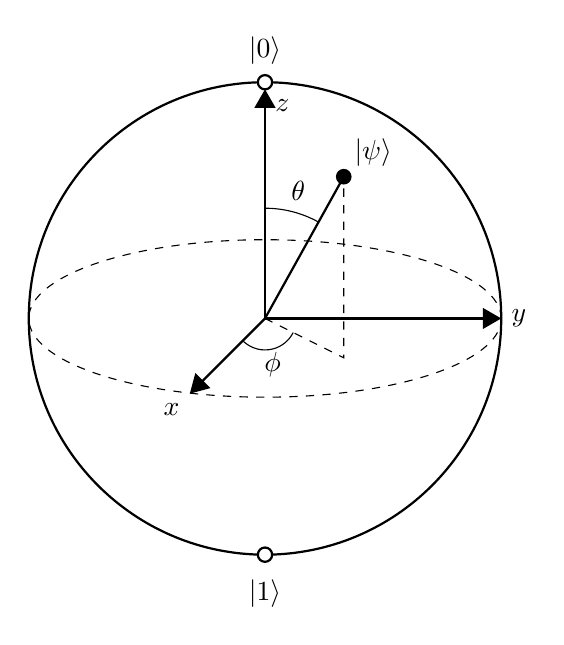
\begin{tikzpicture}

  % Define radius
  \def\r{3}

  \coordinate (orig) at (0,0);
  \coordinate (x) at (-1cm+0.3ex, -1cm+0.3ex);
  \coordinate (y) at (\r, 0);
  \coordinate (z) at (0, 3cm-0.6ex);
  \coordinate (psi) at (\r/3, 3/5*\r);
  \coordinate (phi) at (\r/3, -\r/6);
  \coordinate (bot) at (0, 3cm-0.6ex);

  % Bloch vector
  \draw[thick] (orig) -- (psi) node[circle, fill, inner sep=2, label={[label distance=-3pt]above right:$\ket{\psi}$}] {};
  \draw[dashed] (orig) -- (phi) -- (psi);

  % Sphere
  \draw[thick] (orig) circle (\r);
  \draw[dashed] (orig) ellipse (\r{} and \r/3);

  % Axes
  \draw[thick, -triangle 60] (orig) -- (x) node[below left] {$x$};
  \draw[thick, -triangle 60] (orig) -- (y) node[right] {$y$};
  \draw[thick, -triangle 60] (orig) -- (z) node[below right] {$z$};
  \draw[dashed] (orig) -- (bot);

  % Angles
  \pic [draw=black, "$\phi$", angle eccentricity=1.5, angle radius=0.4cm] {angle = x--orig--phi};
  \pic [draw=black, "$\theta$", angle eccentricity=1.2, angle radius=1.4cm] {angle = psi--orig--z};

  % Ket
  \draw[thick, fill=white] (0,\r) circle (.6ex);
  \draw[thick, fill=white] (0,-\r) circle (.6ex);
  \node at (0,\r+0.4) {$\ket{0}$};
  \node at (0,-\r-0.5) {$\ket{1}$};

\end{tikzpicture}

  \end{center}
  \caption{Bloch sphere representation of a qubit.
    The north pole $(\theta=0)$ is $\ket{0}$, the south pole $(\theta=\pi)$ is $\ket{1}$, and all points on the equator are equal superpositions with varying relative phases.
    The states $\ket{+}$ and $\ket{-}$ sit on the positive and negative $x$-axis; rotations around each axis correspond to specific single-qubit gates.
  }
\end{figure}

Key points on the Bloch sphere:
\begin{center}
  \renewcommand{\arraystretch}{1.3}
  \begin{tabular}{l|c|c}
    \textbf{Axis} & \textbf{$+$ pole} & \textbf{$-$ pole} \\
    \hline
    $z$ & $\ket{0}$ & $\ket{1}$ \\
    $x$ & $\ket{+}=\frac{\ket{0}+\ket{1}}{\sqrt{2}}$ & $\ket{-}=\frac{\ket{0}-\ket{1}}{\sqrt{2}}$ \\
    $y$ & $\ket{i}=\frac{\ket{0}+i\ket{1}}{\sqrt{2}}$ & $\ket{-i}=\frac{\ket{0}-i\ket{1}}{\sqrt{2}}$ \\
  \end{tabular}
\end{center}

Single-qubit unitary gates act as \emph{rotations} of the Bloch sphere.
This geometric picture is very helpful for intuition.

\begin{exercise*}[Measurement probability along arbitrary axis $\vec{v}$]
  A qubit is prepared in $\ket{0}_z$ (the $+1$ eigenstate of $Z$).
  Given a unit vector $\vec{v}=(v_x,v_y,v_z)$ with $\|\vec{v}\|=1$,
  the corresponding spin operator is $\sigma_{\vec{v}}=v_x X+v_y Y+v_z Z$.
  What is the probability of measuring $\ket{0}_{\vec{v}}$ (eigenvalue $+1$)?

  \textbf{Method 1: direct eigenvector.}
  Writing $\vec{v}$ in spherical coordinates ($\theta$ polar, $\phi$ azimuthal):
  $v_x=\sin\theta\cos\phi$, $v_y=\sin\theta\sin\phi$, $v_z=\cos\theta$,
  the matrix of $\sigma_{\vec{v}}$ is
  \begin{equation*}
    \sigma_{\vec{v}} = \begin{bmatrix}v_z & v_x-iv_y \\ v_x+iv_y & -v_z\end{bmatrix}
    = \begin{bmatrix}\cos\theta & \sin\theta\,e^{-i\phi} \\ \sin\theta\,e^{i\phi} & -\cos\theta\end{bmatrix}.
  \end{equation*}
  Solving for the $+1$ eigenvector gives
  $\ket{0}_{\vec{v}} = \cos\tfrac{\theta}{2}\ket{0}+e^{i\phi}\sin\tfrac{\theta}{2}\ket{1}$.
  The probability is:
  \begin{equation*}
    p = \left|\braket{0_{\vec{v}}}{0_z}\right|^2
      = \left|\begin{bmatrix}\cos\tfrac{\theta}{2} & e^{-i\phi}\sin\tfrac{\theta}{2}\end{bmatrix}
              \begin{bmatrix}1\\0\end{bmatrix}\right|^2
      = \cos^2\!\tfrac{\theta}{2} = \frac{1+\cos\theta}{2} = \frac{1+v_z}{2}.
  \end{equation*}

  \textbf{Method 2: density matrix.}
  The initial state has Bloch vector $\vec{r}=(0,0,1)$ and
  the projector for eigenvalue $+1$ of $\sigma_{\vec{v}}$ is
  $P_+=\tfrac{I+\sigma_{\vec{v}}}{2}$.
Then:
  \begin{equation*}
    p(+1) = \tr(\rho\,P_+) = \tr\!\left(\ket{0}\bra{0}\cdot\frac{I+\sigma_{\vec{v}}}{2}\right)
    = \frac{1+\vec{r}\cdot\vec{v}}{2} = \frac{1+(0,0,1)\cdot(v_x,v_y,v_z)}{2} = \frac{1+v_z}{2}.
  \end{equation*}
  Both methods agree.
As a sanity check: if $\vec{v}=\hat{z}$ then $v_z=1$ and $p=1$;
  if $\vec{v}=-\hat{z}$ then $v_z=-1$ and $p=0$;
  if $\vec{v}$ lies in the $xy$-plane then $v_z=0$ and $p=\tfrac{1}{2}$.
\end{exercise*}

\section{Multi-Qubit}

The state of two qubits lives in $\mathbb{C}^2\otimes\mathbb{C}^2\cong\mathbb{C}^4$, spanned by the four computational basis states $\ket{00},\ket{01},\ket{10},\ket{11}$:
\begin{equation*}
  \ket{\psi}=\alpha\ket{00}+\beta\ket{01}+\gamma\ket{10}+\delta\ket{11},\qquad |\alpha|^2+|\beta|^2+|\gamma|^2+|\delta|^2=1
\end{equation*}
For $n$ qubits the state lives in $\mathbb{C}^{2^n}$ and has $2^n$ amplitudes.
This exponential growth is both the source of quantum computing's potential power and one reason large-scale quantum computers are hard to build.

\subsection{Entangled States}

A two-qubit state is \textbf{separable} (or \emph{product}) if it can be written as $\ket{\psi_A}\otimes\ket{\psi_B}$ for some single-qubit states.
Otherwise, it is \textbf{entangled}.

\begin{example*}[Separable state]
  $\ket{\psi}=\frac{1}{\sqrt{2}}(\ket{0}+\ket{1})\otimes\ket{0} =\frac{\ket{00}+\ket{10}}{\sqrt{2}}$.
  The two qubits are independent: measuring the first (getting 0 or 1 with equal probability) tells you nothing about the second.
\end{example*}

\begin{example*}[Entangled state]
  $\ket{\Phi^+}=\frac{\ket{00}+\ket{11}}{\sqrt{2}}$.
  There are no single-qubit states $\ket{\psi_A},\ket{\psi_B}$ with $\ket{\psi_A}\otimes\ket{\psi_B}=\ket{\Phi^+}$.
  (Proof: if $\ket{\psi_A}=a\ket{0}+b\ket{1}$ and $\ket{\psi_B}=c\ket{0}+d\ket{1}$, then $\ket{\psi_A}\otimes\ket{\psi_B}=ac\ket{00}+ad\ket{01}+bc\ket{10}+bd\ket{11}$.
  For this to equal $\frac{1}{\sqrt{2}}(\ket{00}+\ket{11})$ we need $ad=bc=0$ and $ac=bd=\frac{1}{\sqrt{2}}$, which is impossible.)
  
  Measuring the first qubit in the computational basis gives 0 or 1 with probability $\frac{1}{2}$.
  But whichever outcome is obtained, the second qubit is \emph{instantly} in the same state, no matter how far apart the qubits are.
\end{example*}

A practical separability test for a pure two-qubit state $\ket{\psi}=\sum_{ij}a_{ij}\ket{ij}$ uses the coefficient matrix $M=(a_{ij})$: the state is separable iff $\det M=0$.

The four \textbf{Bell states} (also called EPR pairs) are maximally entangled two-qubit states that form an orthonormal basis for $\mathbb{C}^4$:
\begin{align}\label{bell-states}
  \ket{\Phi^+}&=\frac{\ket{00}+\ket{11}}{\sqrt{2}}, &
  \ket{\Phi^-}&=\frac{\ket{00}-\ket{11}}{\sqrt{2}}, \\
  \ket{\Psi^+}&=\frac{\ket{01}+\ket{10}}{\sqrt{2}}, &
  \ket{\Psi^-}&=\frac{\ket{01}-\ket{10}}{\sqrt{2}}.
\end{align}
They are generated from the computational basis by a Hadamard gate followed by a CNOT (see \autoref{chap:gates}).
Their most striking property is \emph{perfect correlation}: if both qubits of $\ket{\Phi^+}$ are measured in the $Z$ basis, the outcomes are always equal (both 0 or both 1), even though each individual outcome is completely random.

\begin{note}
  The $\sqrt{2}$ denominators are required for normalization.
  Without them the sum $\ket{00}+\ket{11}$ has norm $\sqrt{2}$ (since $\braket{00}{00}+\braket{11}{11}=2$), so dividing by $\sqrt{2}$ gives a unit vector.
\end{note}


\begin{exercise*}[Entanglement of a three-qubit state]
  Let $\ket{\psi}=\tfrac{1}{2}(\ket{000}+\ket{001}-\ket{110}-\ket{111})$.
  Label the qubits $A$, $B$, $C$.
  Determine which subsystems are entangled with their complement and, for the non-entangled ones, write $\ket{\psi}$ as a tensor product.

  \textbf{Step 1: factor out qubit $C$.}
  Group terms by the state of $C$:
  \begin{align*}
    \ket{\psi} &= \tfrac{1}{2}\bigl[(\ket{00}-\ket{11})_A{}_B\ket{0}_C
                              +(\ket{00}-\ket{11})_A{}_B\ket{1}_C\bigr] \\
              &= \tfrac{1}{2}(\ket{00}-\ket{11})_{AB}\otimes(\ket{0}+\ket{1})_C.
  \end{align*}
  This is a product state between $C$ and $AB$, so \textbf{$C$ is not entangled with $AB$}.
  Normalizing: $\ket{\psi}=\ket{\Phi^-}_{AB}\otimes\ket{+}_C$ where $\ket{\Phi^-}=\tfrac{\ket{00}-\ket{11}}{\sqrt{2}}$.

  \textbf{Step 2: entanglement of $A$ with $BC$.}
  Since $\ket{\Phi^-}_{AB}$ is a Bell state (a maximally entangled two-qubit state), $A$ and $B$ are entangled.
  Therefore, $A$ is entangled with the system $BC$ --- one cannot write $\ket{\psi}=\ket{\cdot}_A\otimes\ket{\cdot}_{BC}$.

  \textbf{Step 3: entanglement of $B$ with $AC$.}
  By the same reasoning, since $A$ and $B$ are entangled in $\ket{\Phi^-}_{AB}$, $B$ is also entangled with $AC$.

  \textbf{Summary.}
  \begin{itemize}
    \item $C$ is \emph{not} entangled with $AB$: $\ket{\psi}=\ket{\Phi^-}_{AB}\otimes\ket{+}_C$.
    \item $A$ is entangled with $BC$.
    \item $B$ is entangled with $AC$.
  \end{itemize}
\end{exercise*}

\chapter{Quantum Gates and Circuits}\label{chap:gates}

A \textbf{quantum gate} is a unitary transformation applied to one or more qubits.
Two properties follow immediately from unitarity:
\begin{itemize}
  \item \textbf{Reversibility}: $U^\dagger U=I$, so $U^{-1}=U^\dagger$ always exists.
    Every quantum gate has an inverse.
  \item \textbf{Norm preservation}: $\|U\ket{\psi}\|=\|\ket{\psi}\|$, so probabilities are conserved.
\end{itemize}
These properties are very different from classical gates.
A classical AND gate is not invertible (you cannot recover the inputs from the output), and gates have no notion of \quoted{preserving superposition}.

\subsection{Single-Qubit Gates}

\subsubsection{Pauli Gates}

The three \textbf{Pauli matrices} together with the identity are:
\begin{equation*}
  I=\begin{bmatrix}1&0\\0&1\end{bmatrix},\quad
  X=\begin{bmatrix}0&1\\1&0\end{bmatrix},\quad
  Y=\begin{bmatrix}0&-i\\i&0\end{bmatrix},\quad
  Z=\begin{bmatrix}1&0\\0&-1\end{bmatrix}
\end{equation*}

Their actions on the computational basis are:
\begin{center}
  \renewcommand{\arraystretch}{1.3}
  \begin{tabular}{c|c|c|l}
    \textbf{Gate} & $\ket{0}\to$ & $\ket{1}\to$ & \textbf{Meaning} \\
    \hline
    $X$ & $\ket{1}$ & $\ket{0}$ & Bit flip (quantum NOT) \\
    $Y$ & $i\ket{1}$ & $-i\ket{0}$ & Bit+phase flip \\
    $Z$ & $\ket{0}$ & $-\ket{1}$ & Phase flip \\
  \end{tabular}
\end{center}

Key identities: $X^2=Y^2=Z^2=I$; $XY=iZ$; $YZ=iX$; $ZX=iY$; and $\{X,Z\}=XZ+ZX=0$ (they anti-commute).
Any single-qubit operator can be written as $aI+bX+cY+dZ$ for complex scalars $a,b,c,d$.

\begin{exercise*}[Eigenstates of $\sigma_y$]
  Find the eigenvalues and eigenvectors of $\sigma_y$, then express the eigenstates in terms of the $z$-basis states $\ket{0},\ket{1}$.

  \textbf{Eigenvalues.}
  We solve $\det(\sigma_y-\lambda I)=0$:
  \begin{align*}
    \det\!\left(\begin{bmatrix}-\lambda&-i\\i&-\lambda\end{bmatrix}\right)
    &= (-\lambda)^2 - (-i)(i) = \lambda^2 + i^2 = \lambda^2 - 1 = 0
  \end{align*}
  so $\lambda = \pm 1$.

  \textbf{Eigenvector for $\lambda=+1$.}
  We need $\sigma_y\ket{\psi}=\ket{\psi}$ with $\ket{\psi}=\begin{bmatrix}a\\b\end{bmatrix}$:
  \begin{equation*}
    \begin{bmatrix}0&-i\\i&0\end{bmatrix}\begin{bmatrix}a\\b\end{bmatrix}
    = \begin{bmatrix}-ib\\ai\end{bmatrix}
    = \begin{bmatrix}a\\b\end{bmatrix}
    \implies -ib = a.
  \end{equation*}
  Setting $a=1$ gives $b=i$, and the unnormalized eigenvector is $\begin{bmatrix}1\\i\end{bmatrix}$.
  Its norm is $\sqrt{|1|^2+|i|^2}=\sqrt{1+i^*\cdot i}=\sqrt{1+1}=\sqrt{2}$, so:
  \begin{equation*}
    \ket{+y} = \frac{1}{\sqrt{2}}\begin{bmatrix}1\\i\end{bmatrix}
             = \frac{\ket{0}+i\ket{1}}{\sqrt{2}}
             = \frac{\ket{+_z}+i\ket{-_z}}{\sqrt{2}}.
  \end{equation*}

  \textbf{Eigenvector for $\lambda=-1$.}
  Same procedure with $\sigma_y\ket{\psi}=-\ket{\psi}$: one gets $b=-i$ for $a=1$, giving norm $\sqrt{1+(-i)^*(- i)}=\sqrt{1-i^2}=\sqrt{2}$.
  Hence:
  \begin{equation*}
    \ket{-y} = \frac{1}{\sqrt{2}}\begin{bmatrix}1\\-i\end{bmatrix}
             = \frac{\ket{0}-i\ket{1}}{\sqrt{2}}
             = \frac{\ket{+_z}-i\ket{-_z}}{\sqrt{2}}.
  \end{equation*}

  Note that the $\sigma_x$ eigenstates $\ket{\pm x}$ have the same form but without the factor of $i$.
\end{exercise*}

\subsubsection{Hadamard Gate}

\begin{equation*}
  H=\frac{1}{\sqrt{2}}\begin{bmatrix}1&1\\1&-1\end{bmatrix}
\end{equation*}

The Hadamard gate converts between the $Z$-basis ($\ket{0},\ket{1}$) and the $X$-basis ($\ket{+},\ket{-}$):
\begin{equation*}
  H\ket{0}=\ket{+},\quad H\ket{1}=\ket{-},\quad H\ket{+}=\ket{0},\quad H\ket{-}=\ket{1}
\end{equation*}

It is both unitary and Hermitian ($H^\dagger=H$), so $H^2=I$.
Geometrically it is a $180^\circ$ rotation around the diagonal axis halfway between the $x$ and $z$ axes.
The Hadamard gate is the single most important gate in quantum computing: it creates superpositions and enables interference.

\subsubsection{Phase Gates (S and T)}

\begin{equation*}
  S=\begin{bmatrix}1&0\\0&i\end{bmatrix},\qquad
  T=\begin{bmatrix}1&0\\0&e^{i\pi/4}\end{bmatrix}
\end{equation*}

Both leave $\ket{0}$ unchanged and multiply $\ket{1}$ by a phase.
Note $S=T^2$ and $Z=S^2$.
The $T$ gate plays a special role: together with $H$ and CNOT it forms a \emph{universal gate set}.

\subsubsection{Rotation Gates}

For any axis direction $\hat n$ and angle $\theta$, the rotation $R_{\hat n}(\theta)=e^{-i\theta\hat n\cdot\vec\sigma/2}$ is a valid single-qubit gate.
The three standard rotations are:
\begin{equation*}
  R_x(\theta)=\begin{bmatrix}\cos\frac\theta2&-i\sin\frac\theta2\\-i\sin\frac\theta2&\cos\frac\theta2\end{bmatrix},\quad
  R_z(\theta)=\begin{bmatrix}e^{-i\theta/2}&0\\0&e^{i\theta/2}\end{bmatrix}
\end{equation*}

Note $R_z(\pi)=iZ$, $R_z(\pi/2)=e^{i\pi/4}S$, $R_z(\pi/4)=e^{i\pi/8}T$ (up to global phase).

\subsection{Two-Qubit Gates}

\subsubsection{CNOT (Controlled-NOT)}

\begin{equation*}
  \mathrm{CNOT}=\begin{bmatrix}1&0&0&0\\0&1&0&0\\0&0&0&1\\0&0&1&0\end{bmatrix}
\end{equation*}

The CNOT gate has a \textbf{control} qubit and a \textbf{target} qubit.
It flips the target iff the control is $\ket{1}$:
\begin{equation*}
  \ket{c,t}\;\longrightarrow\;\ket{c,\, t\oplus c}
\end{equation*}
The top-left $2\times2$ block is $I$ (control $=0$, target unchanged) and the bottom-right block is $X$ (control $=1$, target flipped).

\begin{figure}[H]
  \centering
  \begin{quantikz}[thin lines, transparent]
  \lstick{$\ket{A}$} & \ctrl{1} & \rstick{$\ket{A}$} \\
  \lstick{$\ket{B}$} & \targ{} & \rstick{$\ket{B \xor A}$}
\end{quantikz}

  \caption{Circuit symbol for the CNOT gate.
    The filled circle on the top wire is the control; the $\oplus$ symbol on the bottom wire is the target.
  }
\end{figure}

\begin{example*}[Generating a Bell state]
  Start from $\ket{00}$:
  \begin{equation*}
    \ket{00} \xrightarrow{H\otimes I} \frac{\ket{0}+\ket{1}}{\sqrt{2}}\otimes\ket{0}
    =\frac{\ket{00}+\ket{10}}{\sqrt{2}} \xrightarrow{\mathrm{CNOT}} \frac{\ket{00}+\ket{11}}{\sqrt{2}}=\ket{\Phi^+}
  \end{equation*}
  The Hadamard creates a superposition on the control; the CNOT entangles the two qubits by conditionally copying the superposition.
\end{example*}

\subsubsection{The Oracle Gate $U_f$}

Many quantum algorithms use a black-box \textbf{oracle} for a function $f:\{0,1\}^n\to\{0,1\}^m$.
The quantum oracle is the unitary:
\begin{equation*}
  U_f\ket{x}\ket{y}=\ket{x}\ket{y\oplus f(x)}
\end{equation*}
This is reversible by construction (applying $U_f$ twice returns the original state, since $y\oplus f(x)\oplus f(x)=y$).
When $m=1$ and $\ket{y}=\ket{0}$, it simply computes $f(x)$ into the ancilla qubit.

\subsubsection{Toffoli Gate (CCNOT)}

The \textbf{Toffoli gate} has two control qubits and one target.
It flips the target iff both controls are $\ket{1}$:
\begin{equation*}
  \ket{a,b,c}\;\longrightarrow\;\ket{a,b,\,c\oplus(a\cdot b)}
\end{equation*}

\begin{figure}[H]
  \begin{minipage}{0.48\textwidth}
    \centering
    \begin{tabular}{ccc|ccc}
      \multicolumn{3}{c}{\textbf{Input}} & \multicolumn{3}{c}{\textbf{Output}} \\
      $a$ & $b$ & $c$ & $a$ & $b$ & $c$ \\
      \hline
      0 & 0 & 0 & 0 & 0 & 0 \\
      0 & 0 & 1 & 0 & 0 & 1 \\
      0 & 1 & 0 & 0 & 1 & 0 \\
      0 & 1 & 1 & 0 & 1 & 1 \\
      1 & 0 & 0 & 1 & 0 & 0 \\
      1 & 0 & 1 & 1 & 0 & 1 \\
      1 & 1 & 0 & 1 & 1 & 1 \\
      1 & 1 & 1 & 1 & 1 & 0 \\
    \end{tabular}
  \end{minipage}
  \begin{minipage}{0.48\textwidth}
    \centering
    \begin{quantikz}[thin lines, transparent]
  \lstick{a} & \ctrl{2} & \rstick{a} \\
  \lstick{b} & \control{} & \rstick{b} \\
  \lstick{c} & \targ{} & \rstick{$\text{c}\xor\text{ab}$}
\end{quantikz}

  \end{minipage}
  \caption{Truth table and circuit symbol for the Toffoli gate.}
\end{figure}

The Toffoli gate is \textbf{classically universal}: setting $c=0$ gives $\ket{a,b,a\cdot b}$ (AND gate), and setting $b=1, c=0$ gives $\ket{a,1,a}$ (fanout, copying bit $a$).
Since NAND and fanout suffice to build any classical circuit, any classical computation can be embedded in a quantum circuit using only Toffoli gates.

\subsection{Universal Gate Sets}

\begin{theorem*}
  Any multiple-qubit gate can be decomposed into single-qubit gates and CNOT gates.
\end{theorem*}

A \textbf{universal gate set} allows approximation of any unitary to arbitrary precision.
The discrete set $\{H, T, \mathrm{CNOT}\}$ is universal (by the Solovay-Kitaev theorem, any unitary can be approximated to error $\varepsilon$ using $O(\log^c(1/\varepsilon))$ gates).

\section{Quantum Circuits}

A \textbf{quantum circuit} is a sequence of quantum gates applied to an initial register of qubits.
Time flows left to right; horizontal wires carry qubits; vertical connections indicate multi-qubit gates.

\begin{center}
  \begin{tabular}{ll}
    \textbf{No loops} & circuits are acyclic (time-ordered) \\
    \textbf{No fan-in} & two wires cannot merge \\
    \textbf{No fan-out} & a wire cannot split (no-cloning, see below) \\
  \end{tabular}
\end{center}

\begin{example*}[Swap circuit]
  Three CNOTs suffice to swap two qubits without ancilla:
  \begin{center}
    \begin{quantikz}[thin lines,transparent, row sep=0.6cm]
  \lstick{$\ket{a}$} & \ctrl{1} & \targ{} & \ctrl{1} & \rstick{$\ket{b}$} \\
  \lstick{$\ket{b}$} & \targ{} & \ctrl{-1} & \targ{} & \rstick{$\ket{a}$}
\end{quantikz}\quad \equiv \quad\begin{quantikz}[thin lines,transparent, row sep=0.9cm]
 \lstick{$\ket{a}$} & \swap{1} & \rstick{$\ket{b}$} \\
 \lstick{$\ket{b}$} & \targX{} & \rstick{$\ket{a}$}
\end{quantikz}

  \end{center}
  The algebra:
  $\ket{a,b}\to\ket{a,a\oplus b}\to\ket{b,a\oplus b}\to\ket{b,a}$.
\end{example*}

\begin{example*}[Bell measurement circuit]
  The inverse of Bell-state preparation: apply CNOT then $H$ to the first qubit, then measure both.
  The four computational-basis outcomes correspond bijectively to the four Bell states.
  This circuit is used in both quantum teleportation and superdense coding.
\end{example*}

\begin{theorem*}[No-cloning]
  There is no unitary $U$ such that $U\ket{\psi}\ket{0}=\ket{\psi}\ket{\psi}$ for all qubit states $\ket{\psi}$.
\end{theorem*}

\begin{proof*}
  Suppose such a $U$ existed.
  For the computational basis states we would need $U\ket{0}\ket{0}=\ket{00}$ and $U\ket{1}\ket{0}=\ket{11}$.
  Now take $\ket{\psi}=\frac{\ket{0}+\ket{1}}{\sqrt{2}}$.
  Linearity of $U$ gives
  \begin{equation*}
    U\ket{\psi}\ket{0}=\frac{\ket{00}+\ket{11}}{\sqrt{2}}
  \end{equation*}
  but the desired output is
  \begin{equation*}
    \ket{\psi}\ket{\psi}=\frac{\ket{00}+\ket{01}+\ket{10}+\ket{11}}{2}
  \end{equation*}
  These are not equal, so $U$ cannot exist.
\end{proof*}

No-cloning has major implications: eavesdropping on a quantum channel necessarily disturbs the signal, enabling the detection of interception (the basis of quantum cryptography).

\section{Quantum Parallelism}

Applying the Hadamard transform to $n$ zero qubits yields the uniform superposition over all $2^n$ bit strings:
\begin{equation*}
  H^{\otimes n}\ket{0}^{\otimes n}=\frac{1}{\sqrt{2^n}}\sum_{x=0}^{2^n-1}\ket{x}
\end{equation*}

Applying an oracle $U_f$ to this superposition gives:
\begin{equation*}
  U_f\!\left(\frac{1}{\sqrt{2^n}}\sum_x\ket{x}\right)\!\ket{0} =\frac{1}{\sqrt{2^n}}\sum_x\ket{x}\ket{f(x)}
\end{equation*}
The single oracle application has \quoted{evaluated $f$ at all $2^n$ inputs simultaneously}.
This is \textbf{quantum parallelism}.

\begin{note}
  The catch is measurement: measuring this state collapses it to a single $\ket{x}\ket{f(x)}$ pair, giving no more information than one classical query.
  The art of quantum algorithms is applying additional gates \emph{before} measuring to extract a \emph{global} property of $f$ (like whether it is constant or balanced) that would take many classical queries to determine.
\end{note}

\textbf{Interference} is the mechanism that makes this useful.
By choosing gates that amplify amplitudes corresponding to correct answers and cancel amplitudes corresponding to wrong ones (like waves cancelling each other), quantum algorithms extract exponentially more information per measurement than classical algorithms can.

\chapter{Quantum Mechanics}

This chapter gives the postulates of quantum mechanics and develops the formalism used to describe open (noisy) quantum systems.

Quantum mechanics emerged from three experimental puzzles that classical physics could not explain:
\begin{itemize}
  \item \textbf{Black-body radiation}: a hot object emits radiation at all frequencies; classically this implies infinite total power (the \quoted{ultraviolet catastrophe}).
    Planck resolved it in 1900 by postulating that energy is \emph{quantized}: a mode of frequency $\nu$ can only exchange energy in discrete packets $E=h\nu$, where $h$ is Planck's constant.
  \item \textbf{Photoelectric effect}: shining light on a metal ejects electrons, but only if the frequency exceeds a threshold (regardless of intensity).
    Einstein (1905) explained this by treating light as composed of \emph{photons}, each carrying energy $h\nu$.
  \item \textbf{Atomic spectra}: hydrogen emits light only at discrete wavelengths.
    Bohr's model (and later Schr\"{o}dinger's wave mechanics) explained this via discrete energy levels $E_n=-13.6/n^2\,\mathrm{eV}$.
\end{itemize}

The key lesson: \emph{energy is quantized, not continuous}.
This quantization is the origin of the word \quoted{quantum}.

\section{The Four Postulates}

\begin{postulate}[State space]
  Any isolated physical system is associated with a Hilbert space $\mathcal{H}$ called the \emph{state space}.
  The system is completely described by a unit vector $\ket{\psi}\in\mathcal{H}$, its \emph{state vector}.
\end{postulate}

The simplest system is a qubit: $\mathcal{H}=\mathbb{C}^2$ with orthonormal basis $\{\ket{0},\ket{1}\}$.

\begin{postulate}[Dynamics / time evolution]
  The time evolution of a closed quantum system is described by the \textbf{Schr\"{o}dinger equation}:
  \begin{equation*}
    i\hbar\frac{d\ket{\psi}}{dt}=H\ket{\psi}
  \end{equation*}
  where $H$ is the \emph{Hamiltonian} (a Hermitian operator) and $\hbar=h/(2\pi)$ is the reduced Planck constant.
  Equivalently, $\ket{\psi(t)}=U(t)\ket{\psi(0)}$ where $U(t)=e^{-iHt/\hbar}$ is a unitary operator.
\end{postulate}

In the quantum circuit model we work with discrete time steps, and each gate is a unitary $U$.
The postulate tells us that any such gate can, in principle, be physically implemented by choosing the right Hamiltonian $H$ and letting the system evolve for the right time.

\begin{postulate}[Observables]
  Any physically measurable quantity (position, energy, spin, \ldots) is represented by a Hermitian operator $M$ on $\mathcal{H}$, called an \emph{observable}.
\end{postulate}

Common examples: energy $\leftrightarrow H$ (Hamiltonian); $z$-spin $\leftrightarrow\sigma_z=Z$; position $\leftrightarrow\hat x$.
Eigenvalues of $M$ are the possible measurement outcomes (and they are real, as required for physical quantities).

\subsection{Heisenberg Uncertainty Principle}

Two observables $A$ and $B$ are said to \textbf{commute} if $[A,B]=AB-BA=0$; they can then be simultaneously diagonalized and measured simultaneously with arbitrary precision.
If they do not commute, there is a fundamental trade-off:

\begin{theorem*}[Robertson uncertainty relation]
  For any state $\ket\psi$ and Hermitian observables $A,B$:
  \begin{equation*}
    \Delta A \cdot \Delta B \ge \frac{1}{2}\bigl|\langle[A,B]\rangle\bigr|
  \end{equation*}
  where $\Delta A=\sqrt{\langle A^2\rangle-\langle A\rangle^2}$ is the standard deviation of $A$.
\end{theorem*}

The most famous instance uses position $\hat x$ and momentum $\hat p$, which satisfy $[\hat x,\hat p]=i\hbar$:
\begin{equation*}
  \Delta x \cdot \Delta p \ge \frac{\hbar}{2}
\end{equation*}
This is the \textbf{Heisenberg uncertainty principle}.
It is not a statement about measurement disturbance; it is a fundamental property of quantum states: no state can simultaneously have a sharp position and a sharp momentum.

\begin{example*}[Energy-time uncertainty]
  A related (but conceptually different) relation is $\Delta E\cdot\Delta t\ge\hbar/2$, where $\Delta t$ is the characteristic time over which the state changes appreciably.
  For a qubit in a superposition of two energy eigenstates with splitting $\Delta E$, this gives the oscillation period $T\sim\hbar/\Delta E$, \ie, the faster the energy splitting, the faster the state oscillates.
  This directly governs gate speeds in physical quantum computers.
\end{example*}

\begin{postulate}[Measurement]
  Let $M=\sum_m m\,P_m$ be the spectral decomposition of an observable ($P_m$ projects onto the eigenspace of eigenvalue $m$).
  Measuring $M$ on state $\ket{\psi}$:
  \begin{itemize}
    \item gives outcome $m$ with probability $p(m)=\bra{\psi}P_m\ket{\psi}$;
    \item after the measurement, the state collapses to
      $P_m\ket{\psi}/\sqrt{p(m)}$.
  \end{itemize}
  The \emph{expectation value} of $M$ is $\langle M\rangle=\sum_m m\,p(m)=\bra{\psi}M\ket{\psi}$.
\end{postulate}

\begin{postulate}[Composite systems]
  The state space of a composite system $AB$ is the tensor product $\mathcal{H}_A\otimes\mathcal{H}_B$.
  If $A$ is in state $\ket{\psi_A}$ and $B$ in state $\ket{\psi_B}$, the joint state is
  $\ket{\psi_A}\otimes\ket{\psi_B}$.
  (Entangled states cannot be written this way.)
\end{postulate}

\begin{example*}[Particle in a box]
  Consider a quantum particle confined between walls at $x=0$ and $x=L$ (infinite potential outside).
  Solving the Schr\"{o}dinger equation gives wave functions $\psi_n(x)=\sqrt{2/L}\sin(n\pi x/L)$ with energies $E_n=n^2\pi^2\hbar^2/(2mL^2)$, $n=1,2,3,\ldots$
  
  Key contrasts with classical mechanics:
  \begin{itemize}
    \item \textbf{Quantized energy}: only discrete levels $E_n$ are allowed; the particle cannot have arbitrary energy;
    \item \textbf{Zero-point energy}: $E_1>0$; the particle can never be at rest;
    \item \textbf{Spatial nodes}: for energy level $n$, there are $n-1$ points where the particle is \emph{never} found (the wave function is zero there).
  \end{itemize}
\end{example*}

\section{General Measurements}

The postulate above describes \textbf{projective measurement} (the most common kind).
A more general formalism is needed to describe partial measurements or measurements of composite systems.

A \textbf{general measurement} is described by operators $\{M_m\}$ (one per outcome) satisfying the \textbf{completeness relation}:
\begin{equation*}
  \sum_m M_m^\dagger M_m = I
\end{equation*}
Measuring $\{M_m\}$ on state $\ket{\psi}$:
\begin{equation*}
  p(m)=\bra{\psi}M_m^\dagger M_m\ket{\psi},\qquad \ket{\psi}\to\frac{M_m\ket{\psi}}{\sqrt{p(m)}}
\end{equation*}
Projective measurement is the special case $M_m=P_m$ (orthogonal projectors: $P_m^2=P_m$, $P_mP_{m'}=\delta_{mm'}P_m$).
An important property of projective measurements is \textbf{repeatability}: a second measurement immediately after the first gives the same outcome with certainty (the state is already in the eigenspace $P_m$).

\begin{exercise*}[Probability of outcome 0]
  Given $\ket{\psi}=\alpha\ket{0}+\beta\ket{1}$, compute $p(0)$ using the projector $P_0=\ket{0}\bra{0}$.
  \begin{align*}
    p(0)&=\bra{\psi}P_0^\dagger P_0\ket{\psi}=\bra{\psi}P_0\ket{\psi}
        =\bra{\psi}\ket{0}\braket{0}{\psi}=|\braket{0}{\psi}|^2=|\alpha|^2
  \end{align*}
\end{exercise*}

\subsection{POVM}

A \textbf{Positive Operator-Valued Measure} (POVM) describes what outcomes are possible and with what probability, without specifying the post-measurement state.
It is a set of positive operators $\{E_m\}$ with $\sum_m E_m=I$; the outcome probabilities are $p(m)=\bra{\psi}E_m\ket{\psi}$.

POVMs are useful when we care only about the statistics of outcomes (\eg, in cryptographic protocols where the goal is to distinguish two non-orthogonal states).

\begin{example*}[Distinguishing non-orthogonal states with a POVM]
  Alice prepares either $\ket{0}$ or $\ket{+}=\frac{\ket{0}+\ket{1}}{\sqrt{2}}$ with equal probability.
  No projective measurement can always distinguish them, but the three-element POVM
  \begin{equation*}
    E_1=\frac{\sqrt{2}}{1+\sqrt{2}}\ket{1}\bra{1},\quad
    E_2=\frac{\sqrt{2}}{1+\sqrt{2}}\ket{-}\bra{-},\quad
    E_3=I-E_1-E_2
  \end{equation*}
  has the property that outcome 1 never occurs for $\ket{0}$ (ruling out $\ket{+}$), and outcome 2 never occurs for $\ket{+}$ (ruling out $\ket{0}$).
  When outcome 3 occurs, the state is inconclusive.
  This is called \emph{unambiguous state discrimination}.
\end{example*}

\section{Density Operator}

So far we have described states as pure vectors $\ket{\psi}$.
In practice there are two distinct situations that force us to go beyond pure states:
\begin{enumerate}
  \item \textbf{Classical uncertainty about preparation}: we prepare state $\ket{\psi_i}$ with probability $p_i$ but do not record which one was actually prepared.
    This is a \emph{statistical mixture}, arising from \emph{lack of knowledge}---a classical source of randomness layered on top of the quantum state.
  \item \textbf{Entanglement with an inaccessible system}: the system of interest is one part of a larger entangled state; after tracing out the rest, the reduced state is genuinely mixed, not merely a result of ignorance.
    This is a fundamentally quantum source of mixedness.
\end{enumerate}
Both situations are captured by the \textbf{density operator}:
\begin{equation*}
  \rho=\sum_i p_i\ket{\psi_i}\bra{\psi_i}
\end{equation*}
where $p_i\ge0$, $\sum_i p_i=1$, and the $\ket{\psi_i}$ need not be orthogonal.
This is called an \emph{ensemble} decomposition of $\rho$.

\begin{note}
  The ensemble decomposition is \emph{not unique}: the same density operator $\rho$ can be written as a mixture of many different ensembles.
  For example, $\frac{I}{2}=\frac12\ket{0}\bra{0}+\frac12\ket{1}\bra{1} =\frac12\ket{+}\bra{+}+\frac12\ket{-}\bra{-}$.
  No experiment on the system alone can distinguish these preparations; $\rho$ contains all physically accessible information.
\end{note}

\begin{theorem*}[Characterisation]
  An operator $\rho$ is a valid density operator iff:
  \begin{itemize}
    \item $\tr(\rho)=1$ \quad(probabilities sum to 1);
    \item $\rho\ge 0$ \quad(positive semidefinite).
  \end{itemize}
\end{theorem*}

\subsection{Spectral Decomposition}

Since $\rho$ is positive semidefinite it is Hermitian, so the spectral theorem applies.
There always exists an orthonormal basis of eigenvectors $\ket{e_i}$ with real non-negative eigenvalues $\lambda_i$ summing to 1:
\begin{equation*}
  \rho = \sum_i \lambda_i \ket{e_i}\bra{e_i}, \qquad \lambda_i \ge 0,\quad \sum_i\lambda_i = 1
\end{equation*}
This is the \emph{canonical} ensemble decomposition using orthogonal states, and it is \emph{unique} when all eigenvalues are distinct.

\textbf{Pure vs mixed states}: Since the $\lambda_i$ are non-negative and sum to 1, we have
\begin{equation*}
  \tr(\rho^2)=\sum_i\lambda_i^2 \le \left(\sum_i\lambda_i\right)^2 = 1
\end{equation*}
with equality iff exactly one $\lambda_i=1$ and the rest are zero, \ie, iff $\rho=\ket{\psi}\bra{\psi}$ for some $\ket{\psi}$.
So:
\begin{itemize}
  \item $\rho$ is a \textbf{pure state} $\iff$ $\rho^2=\rho$ $\iff$ $\tr(\rho^2)=1$ $\iff$ $\rho=\ket\psi\bra\psi$ for some $\ket\psi$;
  \item $\rho$ is a \textbf{mixed state} $\iff$ $\tr(\rho^2)<1$ $\iff$ more than one $\lambda_i$ is nonzero.
\end{itemize}

\subsection{Measurement Rules}

The density operator obeys the following rules, which parallel the postulates for pure states:
\begin{itemize}
  \item \textbf{Unitary evolution}: $\rho \to U\rho U^\dagger$.
    (Proof: if $\rho=\sum_i p_i\ket{\psi_i}\bra{\psi_i}$ then $U\rho U^\dagger=\sum_i p_i U\ket{\psi_i}\bra{\psi_i}U^\dagger$, which is the density operator of the evolved ensemble.)
  \item \textbf{Measurement probability}: $p(m)=\tr(M_m^\dagger M_m\,\rho)$.
  \item \textbf{Post-measurement state}: after obtaining outcome $m$,
    \begin{equation*}
      \rho \;\to\; \rho_m = \frac{M_m\,\rho\,M_m^\dagger}{\tr(M_m^\dagger M_m\,\rho)}
    \end{equation*}
    For a projective measurement ($M_m=P_m$) this simplifies to $\rho_m = P_m\rho P_m / p(m)$.
\end{itemize}

\begin{example*}[Verifying the measurement probability formula]
  For a pure state $\rho=\ket\psi\bra\psi$ and projector $P_m$:
  \begin{equation*}
    \tr(P_m\rho) = \tr(P_m\ket\psi\bra\psi) = \bra\psi P_m\ket\psi = p(m)
  \end{equation*}
  where we used cyclicity of trace: $\tr(P_m\ket\psi\bra\psi)=\tr(\bra\psi P_m\ket\psi)=\bra\psi P_m\ket\psi$.
\end{example*}

\begin{example*}[Bloch vector representation]
  Any single-qubit density matrix can be written as
  \begin{equation*}
    \rho=\frac{1}{2}(I+r_x X+r_y Y+r_z Z)
  \end{equation*}
  where $(r_x,r_y,r_z)\in\mathbb{R}^3$ is the \emph{Bloch vector}.
  The state is pure iff $|\vec r|=1$ (on the sphere surface), mixed iff $|\vec r|<1$ (inside the sphere).
  The maximally mixed state $\rho=\frac{I}{2}$ sits at the center $\vec r=\vec 0$.

  Explicitly, for a pure state
  $\ket\psi=\cos\frac\theta2\ket0+e^{i\phi}\sin\frac\theta2\ket1$:
  \begin{equation*}
    \rho=\ket\psi\bra\psi=\frac12\begin{bmatrix}1+\cos\theta & e^{-i\phi}\sin\theta \\ e^{i\phi}\sin\theta & 1-\cos\theta\end{bmatrix}
  \end{equation*}
  so $r_x=\sin\theta\cos\phi$, $r_y=\sin\theta\sin\phi$, $r_z=\cos\theta$---precisely the Bloch sphere spherical coordinates.
\end{example*}

\subsection{Reduced Density Operator and Partial Trace}

Given a composite system $AB$ in state $\rho^{AB}$, the \textbf{reduced density operator} of subsystem $A$ is obtained by \emph{tracing out} system $B$:
\begin{equation*}
  \rho^A=\tr_B(\rho^{AB})=\sum_k\bra{k}_B\,\rho^{AB}\,\ket{k}_B
\end{equation*}
where $\{\ket{k}_B\}$ is any orthonormal basis of $\mathcal{H}_B$.
The result is independent of which basis is used.
This gives the correct probability for any measurement performed on $A$ alone: $p(m)=\tr_A(M_m^\dagger M_m\,\rho^A)$.

\begin{example*}[Partial trace computed step by step]
  Take $\rho^{AB}=\ket{\Phi^+}\bra{\Phi^+}$ with $\ket{\Phi^+}=\frac{\ket{00}+\ket{11}}{\sqrt{2}}$.
  Using the basis $\{\ket{0}_B,\ket{1}_B\}$:
  \begin{align*}
    \rho^A &= \bra{0}_B\,\rho^{AB}\,\ket{0}_B + \bra{1}_B\,\rho^{AB}\,\ket{1}_B
  \end{align*}
  First term: $\bra{0}_B\ket{\Phi^+}=\frac{1}{\sqrt2}\ket{0}_A$, so $\bra{0}_B\rho^{AB}\ket{0}_B=\frac12\ket0\bra0$.
  Second term: $\bra{1}_B\ket{\Phi^+}=\frac{1}{\sqrt2}\ket{1}_A$, so $\bra{1}_B\rho^{AB}\ket{1}_B=\frac12\ket1\bra1$.
  Therefore:
  \begin{equation*}
    \rho^A=\frac12\ket0\bra0+\frac12\ket1\bra1=\frac{I}{2}
  \end{equation*}
  The reduced state is maximally mixed: measuring $A$ alone gives a completely random result, even though the joint state is pure.
\end{example*}

\textbf{Entanglement characterization via partial trace}: for a \emph{pure} bipartite state $\ket\psi^{AB}$,
\begin{equation*}
  \ket\psi^{AB} \text{ is separable} \iff \rho^A = \tr_B(\ket\psi\bra\psi) \text{ is a pure state}
\end{equation*}
\begin{proof*}
  If $\ket\psi=\ket{a}\ket{b}$ then $\rho^A=\ket{a}\bra{a}$, which is pure.
  Conversely, if $\rho^A$ is pure with Schmidt decomposition $\ket\psi=\sum_i\lambda_i\ket{i_A}\ket{i_B}$ and $\rho^A=\sum_i\lambda_i^2\ket{i_A}\bra{i_A}$, then $\rho^A$ pure requires exactly one nonzero $\lambda_i$, \ie, Schmidt number 1, \ie, $\ket\psi$ separable.
\end{proof*}

\section{Schmidt Decomposition}\label{sec:schmidt}

\begin{theorem*}[Schmidt decomposition]
  For any pure state $\ket{\psi}\in\mathcal{H}_A\otimes\mathcal{H}_B$ there exist orthonormal sets $\{\ket{i_A}\}$, $\{\ket{i_B}\}$ and real non-negative \emph{Schmidt coefficients} $\lambda_i$ with $\sum_i\lambda_i^2=1$ such that
  \begin{equation*}
    \ket{\psi}=\sum_i\lambda_i\ket{i_A}\ket{i_B}
  \end{equation*}
\end{theorem*}

\begin{proof*}
  Write $\ket\psi=\sum_{i,j}a_{ij}\ket{i_A}\ket{j_B}$ in any product basis.
  Let $A=(a_{ij})$ be the matrix of coefficients and apply SVD: $A=UDV^\dagger$, where $U,V$ are unitary and $D$ is diagonal
  with non-negative entries $\lambda_i=D_{ii}$.
  Define new orthonormal bases $\ket{i_A}=\sum_k U_{ki}\ket{k_A}$ and $\ket{i_B}=\sum_l V_{li}\ket{l_B}$.
  Then:
  \begin{equation*}
    \ket\psi=\sum_{ij}a_{ij}\ket{i_A}\ket{j_B} =\sum_{ij}(UDV^\dagger)_{ij}\ket{i_A}\ket{j_B} =\sum_k\lambda_k\ket{k_A}\ket{k_B}
  \end{equation*}
  Normalization: $\sum_k\lambda_k^2=\tr(D^2)=\tr(A^\dagger A)=\sum_{ij}|a_{ij}|^2=1$.
\end{proof*}

\textbf{Relationship to the reduced density operator}: tracing out $B$,
\begin{equation*}
  \rho^A = \tr_B(\ket\psi\bra\psi) = \sum_i\lambda_i^2\ket{i_A}\bra{i_A}
\end{equation*}
so the Schmidt coefficients squared are the \emph{eigenvalues} of $\rho^A$.
Similarly, $\rho^B=\sum_i\lambda_i^2\ket{i_B}\bra{i_B}$, so $\rho^A$ and $\rho^B$ have the same non-zero eigenvalues.

The \textbf{Schmidt number} is the number of non-zero Schmidt coefficients:
\begin{itemize}
  \item Schmidt number $=1$ $\iff$ state is \textbf{separable} (one term: $\ket\psi=\ket{a}\ket{b}$; $\rho^A$ is pure).
  \item Schmidt number $>1$ $\iff$ state is \textbf{entangled} ($\rho^A$ is mixed).
\end{itemize}

\begin{example*}[Separability check via coefficient matrix]
  For a two-qubit state $\ket\psi=\sum_{ij}a_{ij}\ket{ij}$, form the $2\times2$ matrix $M=(a_{ij})$.
  The state is separable iff $\operatorname{rank}(M)=1$, iff $\det(M)=0$.

  Check $\ket\psi=\frac{\ket{00}+\ket{11}}{\sqrt2}$: $M=\frac{1}{\sqrt2}\begin{bmatrix}1&0\\0&1\end{bmatrix}$, $\det M=\frac12\neq0$, so it is \textbf{entangled}.

  Check $\ket\psi=\frac{\ket{00}+\ket{01}}{\sqrt2}$: $M=\frac{1}{\sqrt2}\begin{bmatrix}1&1\\0&0\end{bmatrix}$, $\det M=0$, so it is \textbf{separable} ($=\ket0\otimes\frac{\ket0+\ket1}{\sqrt2}$).
\end{example*}

\begin{example*}[Schmidt coefficients of $\ket{\Phi^+}$]
  $\ket{\Phi^+}=\frac{1}{\sqrt{2}}\ket{0_A0_B}+\frac{1}{\sqrt{2}}\ket{1_A1_B}$ is already in Schmidt form with $\lambda_1=\lambda_2=\frac{1}{\sqrt{2}}$ and Schmidt number 2, so it is maximally entangled for a two-qubit system.
  Its reduced state $\rho^A=\frac12 I$ has maximum entropy $S(\rho^A)=-\tr(\rho^A\log\rho^A)=\log 2=1$ ebit.
\end{example*}

\begin{exercise*}[Checking entanglement via the coefficient matrix]
  Determine which of the following two-qubit states are entangled:
  \begin{align*}
    \ket{\phi_1} &= \tfrac{1}{\sqrt{2}}(\ket{01}-\ket{10}), \\
    \ket{\phi_2} &= \tfrac{1}{2}(\ket{00}+\ket{01}+\ket{10}+\ket{11}), \\
    \ket{\phi_3} &= \tfrac{1}{\sqrt{2a^2+2b^2}}(a\ket{00}+b\ket{01}+b\ket{10}+a\ket{11}).
  \end{align*}

  \textbf{Method.}  Write $\ket{\psi}=\sum_{ij}c_{ij}\ket{ij}$ and form the $2\times2$ coefficient matrix $M_\psi=\begin{bmatrix}c_{00}&c_{01}\\c_{10}&c_{11}\end{bmatrix}$. A state is separable if and only if $\det(M_\psi)=0$.

  \textbf{$\ket{\phi_1}$:}
  $M_{\phi_1}=\begin{bmatrix}0&\frac{1}{\sqrt{2}}\\-\frac{1}{\sqrt{2}}&0\end{bmatrix}$,
  $\det(M_{\phi_1})=0-\bigl(\tfrac{1}{\sqrt{2}}\bigr)(-\tfrac{1}{\sqrt{2}})=\tfrac{1}{2}\neq0$.
  This is the Bell state $\ket{\Psi^-}$, so it is \textbf{entangled}.

  \textbf{$\ket{\phi_2}$:}
  $M_{\phi_2}=\begin{bmatrix}\frac{1}{2}&\frac{1}{2}\\\frac{1}{2}&\frac{1}{2}\end{bmatrix}$,
  $\det(M_{\phi_2})=\tfrac{1}{4}-\tfrac{1}{4}=0$.
  \textbf{Not entangled}: indeed $\ket{\phi_2}=\ket{+}\otimes\ket{+}$.

  \textbf{$\ket{\phi_3}$:}
  $M_{\phi_3}=\frac{1}{\sqrt{2a^2+2b^2}}\begin{bmatrix}a&b\\b&a\end{bmatrix}$,
  $\det(M_{\phi_3})=\frac{a^2-b^2}{2a^2+2b^2}$.
  This is zero iff $a=\pm b$.
  For $a\neq\pm b$ the state is \textbf{entangled}; for $a=b$ it reduces to $\ket{\phi_2}$ (up to normalization) and for $a=-b$ to $\ket{\Phi^-}$ (entangled, matching case 1 above).
\end{exercise*}

\section{Bell Inequality}

Einstein, Podolsky, and Rosen (EPR) argued in 1935 that quantum mechanics is \emph{incomplete}: the \quoted{spooky action at a distance} apparent in entanglement must mean that hidden local variables pre-determine measurement outcomes.
Bell showed in 1964 that hidden-variable theories are testably different from quantum mechanics.

\subsection{CHSH Inequality}

Let Alice choose observable $Q$ or $R$ and Bob choose $S$ or $T$, all with eigenvalues $\pm1$.
Define
\begin{equation*}
  \B=QS+RS+RT-QT
\end{equation*}
For any deterministic assignment of values $q,r,s,t\in\{+1,-1\}$:
\begin{equation*}
  \B=q(s-t)+r(s+t);\quad\text{if }s=t:\B=2r=\pm2;\quad\text{if }s=-t:\B=2q=\pm2
\end{equation*}
So $\B=\pm2$ always, and any local hidden-variable theory predicts $|\langle\B\rangle|\le2$.
This is the \textbf{Bell-CHSH inequality}.

\subsection{Quantum Violation}

For the singlet $\ket{\Psi^-}=\frac{\ket{01}-\ket{10}}{\sqrt{2}}$ and the choices $Q=Z_1$, $R=X_1$, $S=\frac{-Z_2-X_2}{\sqrt{2}}$, $T=\frac{Z_2-X_2}{\sqrt{2}}$, we compute each correlator $E(QS)=\bra{\Psi^-}Q\otimes S\ket{\Psi^-}$.

\begin{example*}[Computing $E(QS)$ explicitly]
  $Q\otimes S = Z_1\otimes\frac{-Z_2-X_2}{\sqrt2}$.
  Using $Z\ket0=\ket0$, $Z\ket1=-\ket1$, $X\ket0=\ket1$, $X\ket1=\ket0$:
  \begin{align*}
    (Z\otimes Z)\ket{\Psi^-} &= Z\otimes Z\cdot\frac{\ket{01}-\ket{10}}{\sqrt2}
    = \frac{-\ket{01}+(-1)(-1)\ket{10}}{\sqrt2} = \frac{-\ket{01}+\ket{10}}{\sqrt2} = -\ket{\Psi^-} \\
    (Z\otimes X)\ket{\Psi^-} &= \frac{Z\ket0\otimes X\ket1-Z\ket1\otimes X\ket0}{\sqrt2}
    = \frac{\ket{00}+\ket{11}}{\sqrt2} = \ket{\Phi^+}
  \end{align*}
  Therefore $E(QS)=\bra{\Psi^-}\frac{-Z\otimes Z-Z\otimes X}{\sqrt2}\ket{\Psi^-} =\frac{-(-1)-0}{\sqrt2}=\frac{1}{\sqrt2}$.
\end{example*}

By symmetry of the chosen angles, $E(RS)=E(RT)=\frac{1}{\sqrt2}$ and $E(QT)=-\frac{1}{\sqrt2}$, giving:
\begin{equation*}
  \langle\B\rangle = E(QS)+E(RS)+E(RT)-E(QT)
  = \frac{1}{\sqrt2}+\frac{1}{\sqrt2}+\frac{1}{\sqrt2}+\frac{1}{\sqrt2}
  = \frac{4}{\sqrt{2}} = 2\sqrt{2}\approx 2.83
\end{equation*}
This violates the classical bound of 2.

\begin{theorem*}[Tsirelson bound]
  For any quantum state and any observables with eigenvalues $\pm1$: $|\langle\B\rangle|\le2\sqrt{2}$.
\end{theorem*}

\begin{proof*}
  Compute $\B^2=(QS+RS+RT-QT)^2$.
  Expanding and using $Q^2=R^2=S^2=T^2=I$, one finds:
  \begin{equation*}
    \B^2 = 4I - [Q,R]\otimes[S,T]
  \end{equation*}
  Taking the expectation value and using the operator norm bound $\|[A,B]\|\le2\|A\|\cdot\|B\|=2$ (since $\|A\|=\|B\|=1$ for $\pm1$-observables):
  \begin{equation*}
    \langle\B^2\rangle\le 4+\|[Q,R]\|\cdot\|[S,T]\|\le 4+2\cdot2=8
  \end{equation*}
  By Cauchy-Schwarz, $\langle\B\rangle^2\le\langle\B^2\rangle\le8$, so $|\langle\B\rangle|\le2\sqrt2$.
  The bound is saturated by the $\ket{\Psi^-}$ construction above.
\end{proof*}

\begin{exercise*}[CHSH violation with $\ket{\Psi^-}$]
  Prove the CHSH inequality $|\B|\le2$ for classical $\pm1$ variables, then show it is violated for the Bell state $\ket{\Psi^-}$ with observables $Q=Z_1$, $R=X_1$, $S=\tfrac{-Z_2-X_2}{\sqrt{2}}$, $T=\tfrac{Z_2-X_2}{\sqrt{2}}$.

  \textbf{Classical bound.}
  For any deterministic assignment $q,r,s,t\in\{+1,-1\}$:
  $\B=qs+rs+rt-qt=s(q+r)+t(r-q)$.
  If $q=r$, then $r-q=0$ and $\B=2rs=\pm2$.
  If $q=-r$, then $q+r=0$ and $\B=2rt=\pm2$.
  So $|\B|\le2$ classically.

  \textbf{Quantum violation.}
  Substituting the operators:
  \begin{align*}
    \B &= QS+RS+RT-QT \\
       &= -Z_1Z_2 - Z_1X_2 - X_1Z_2 - X_1X_2 + X_1Z_2 - X_1X_2 - Z_1Z_2 + Z_1X_2 \\
       &= -2(Z_1Z_2+X_1X_2)/\sqrt{2}
  \end{align*}
  We evaluate the expectation values on $\ket{\Psi^-}=\tfrac{\ket{01}-\ket{10}}{\sqrt{2}}$ using the fact that
  \begin{equation*}
    Z_1Z_2\ket{\Psi^-}=-\ket{\Psi^-} \quad \andt \quad X_1X_2\ket{\Psi^-}=-\ket{\Psi^-}
  \end{equation*}
  , so $\langle Z_1Z_2\rangle=\langle X_1X_2\rangle=-1$.
  Therefore:
  \begin{equation*}
    \langle\B\rangle = -\sqrt{2}\bigl(\langle Z_1Z_2\rangle+\langle X_1X_2\rangle\bigr) = -\sqrt{2}(-1-1) = 2\sqrt{2} > 2.
  \end{equation*}
\end{exercise*}
hold for quantum mechanics:
\begin{enumerate}
  \item \textbf{Non-realism}: properties do not have definite values before measurement.
  \item \textbf{Non-locality}: measurements on one system can instantaneously influence a distant system.
\end{enumerate}
Loophole-free experiments (Hensen et al.\ 2015, among others) have conclusively confirmed the quantum violation $\langle\B\rangle>2$, ruling out all local hidden-variable theories.

\section{Purification}

Given any mixed state $\rho^A=\sum_i p_i\ket{i_A}\bra{i_A}$, we can \textbf{purify} it by introducing a reference system $R$ of the same dimension and defining:
\begin{equation*}
  \ket{AR}=\sum_i\sqrt{p_i}\ket{i_A}\ket{i_R}
\end{equation*}
Then $\tr_R(\ket{AR}\bra{AR})=\rho^A$.
This shows that every mixed state can be viewed as one half of a pure entangled state.
The physical intuition: a mixed state arises from \emph{entanglement with an environment} that we have no access to.

\begin{exercise*}[Purification of a density matrix]
  Describe the purification procedure and apply it to:
  \begin{equation*}
    \rho = \frac{1}{4}\frac{(\ket{0}+\ket{1})(\bra{0}+\bra{1})}{2}
         + \frac{3}{4}\frac{(\ket{0}-\ket{1})(\bra{0}-\bra{1})}{2}
         = \frac{1}{4}\ket{+}\bra{+} + \frac{3}{4}\ket{-}\bra{-}.
  \end{equation*}
  Verify that the partial trace over the auxiliary system recovers $\rho$.

  \textbf{Concept.}
  The purification of a density matrix $\rho_A$ consists in finding a pure state $\ket{\psi_{AB}}$ in a larger composite space (original space $A$ plus auxiliary $B$) such that $\tr_B(\ket{\psi_{AB}}\bra{\psi_{AB}})=\rho_A$.

  \textbf{Spectral decomposition.}
  Since $\braket{+}{-}=0$, the states $\ket{+},\ket{-}$ already form an orthonormal basis, so the above is already the spectral decomposition of $\rho$ with eigenvalues $\lambda_1=\tfrac{1}{4}$, $\lambda_2=\tfrac{3}{4}$ and eigenstates $\ket{\psi_1}_A=\ket{+}$, $\ket{\psi_2}_A=\ket{-}$.

  \textbf{Building the purification.}
  We introduce auxiliary system $B$ with orthonormal basis $\{\ket{0}_B,\ket{1}_B\}$ and define (using the general formula $\ket{\psi_{AB}}=\sum_i\sqrt{\lambda_i}\ket{i_A}\otimes\ket{i_B}$):
  \begin{equation*}
    \ket{\psi_{AB}} = \sqrt{\tfrac{1}{4}}\,\ket{+}_A\ket{0}_B
                    + \sqrt{\tfrac{3}{4}}\,\ket{-}_A\ket{1}_B
    = \frac{1}{2}\ket{+}_A\ket{0}_B + \frac{\sqrt{3}}{2}\ket{-}_A\ket{1}_B.
  \end{equation*}

  \textbf{Verification.}
  We compute $\rho_A = \tr_B(\ket{\psi_{AB}}\bra{\psi_{AB}}) = \sum_{k\in\{0,1\}}{}_B\!\bra{k}\,\rho_{AB}\,\ket{k}_B$:
  \begin{align*}
    \rho_{AB} &= \Bigl(\tfrac{1}{2}\ket{+}_A\ket{0}_B + \tfrac{\sqrt{3}}{2}\ket{-}_A\ket{1}_B\Bigr)
                 \Bigl(\tfrac{1}{2}\bra{+}_A\bra{0}_B + \tfrac{\sqrt{3}}{2}\bra{-}_A\bra{1}_B\Bigr).
  \end{align*}
  Taking the partial trace over $B$, the cross terms vanish because $\braket{0}{1}_B=0$
  and $\braket{1}{0}_B=0$, and the diagonal terms yield:
  \begin{equation*}
    \rho_A = \tfrac{1}{4}\ket{+}\bra{+}\cdot\underbrace{\braket{0}{0}}_B
           + \tfrac{3}{4}\ket{-}\bra{-}\cdot\underbrace{\braket{1}{1}}_B
           = \tfrac{1}{4}\ket{+}\bra{+} + \tfrac{3}{4}\ket{-}\bra{-} = \rho.
  \end{equation*}
\end{exercise*}

\section{Quantum Channels and Noise}

Real quantum systems are never perfectly isolated; they interact with their environment.
The framework that describes the resulting noisy evolution is that of \textbf{quantum channels} (also called completely positive trace-preserving maps, or CPTP maps).

\subsection{Kraus Representation}

\begin{theorem*}[Kraus representation]
  Any quantum channel $\mathcal{E}$ (a physical, trace-preserving
  evolution of a density matrix) can be written as
  \begin{equation*}
    \mathcal{E}(\rho)=\sum_k K_k\rho K_k^\dagger
  \end{equation*}
  where the \textbf{Kraus operators} $K_k$ satisfy the completeness
  condition $\sum_k K_k^\dagger K_k=I$.
\end{theorem*}

Unitary evolution is the special case of a single Kraus operator $K=U$.
The general case handles decoherence, dissipation, and measurement backaction.

\subsection{Important Single-Qubit Noise Channels}

The following channels describe the most common physical errors, and are the errors that quantum error correction must address.

\paragraph{Bit-flip channel.}
With probability $p$ the qubit suffers an $X$ error:
\begin{equation*}
  \mathcal{E}_{\mathrm{bf}}(\rho)=(1-p)\rho+p\,X\rho X
\end{equation*}
Kraus operators: $K_0=\sqrt{1-p}\,I$, $K_1=\sqrt{p}\,X$.

\paragraph{Phase-flip (dephasing) channel.}
With probability $p$ the qubit suffers a $Z$ error:
\begin{equation*}
  \mathcal{E}_{\mathrm{ph}}(\rho)=(1-p)\rho+p\,Z\rho Z
\end{equation*}
In terms of the Bloch vector $(r_x,r_y,r_z)$, this maps $(r_x,r_y,r_z)\to((1-2p)r_x,(1-2p)r_y,r_z)$: the $x$ and $y$ components decay, destroying phase coherence while leaving the $z$ component (the classical bit) intact.
This is the dominant noise process in most real hardware.

\begin{exercise*}[Dephasing applied to a pure qubit]
  Apply the dephasing channel $\mathcal{E}(\rho)=(1-p)\rho+p\,\sigma_z\rho\sigma_z^\dagger$
  to the qubit $\ket{\psi}=\alpha\ket{0}+\beta\ket{1}$.

  \textbf{Density matrix.}
  The pure state density matrix is:
  \begin{equation*}
    \rho = \ket{\psi}\bra{\psi} =
    \begin{bmatrix}|\alpha|^2 & \alpha\beta^* \\ \alpha^*\beta & |\beta|^2\end{bmatrix}.
  \end{equation*}

  \textbf{Applying the channel.}
  We compute $\sigma_z\rho\sigma_z^\dagger$ explicitly:
  \begin{align*}
    \sigma_z\rho\sigma_z &=
    \begin{bmatrix}1&0\\0&-1\end{bmatrix}
    \begin{bmatrix}|\alpha|^2 & \alpha\beta^* \\ \alpha^*\beta & |\beta|^2\end{bmatrix}
    \begin{bmatrix}1&0\\0&-1\end{bmatrix}
    = \begin{bmatrix}|\alpha|^2 & -\alpha\beta^* \\ -\alpha^*\beta & |\beta|^2\end{bmatrix}.
  \end{align*}
  Combining:
  \begin{align*}
    \mathcal{E}(\rho) &= (1-p)\begin{bmatrix}|\alpha|^2 & \alpha\beta^* \\ \alpha^*\beta & |\beta|^2\end{bmatrix}
    + p\begin{bmatrix}|\alpha|^2 & -\alpha\beta^* \\ -\alpha^*\beta & |\beta|^2\end{bmatrix} \\
    &= \begin{bmatrix}|\alpha|^2 & (1-2p)\alpha\beta^* \\ (1-2p)\alpha^*\beta & |\beta|^2\end{bmatrix}.
  \end{align*}
  The diagonal entries (populations) are unchanged, while the off-diagonal entries (coherences) are damped by a factor $(1-2p)$.
At $p=\tfrac{1}{2}$ the coherences vanish entirely and the state becomes fully classical.
\end{exercise*}

\paragraph{Depolarizing channel.}
With probability $p$ the qubit is replaced by the maximally mixed state $I/2$; equivalently, each Pauli error occurs with probability
$p/4$:
\begin{equation*}
  \mathcal{E}_{\mathrm{dep}}(\rho)=\left(1-p\right)\rho+\frac{p}{4}(I\rho I+X\rho X+Y\rho Y+Z\rho Z)
  =\left(1-\frac{3p}{4}\right)\rho+\frac{p}{4}I
\end{equation*}
Bloch vector shrinks uniformly: $(r_x,r_y,r_z)\to(1-p)(r_x,r_y,r_z)$.
The depolarizing channel is a common worst-case noise model in error correction analysis.

\paragraph{Amplitude damping channel.}
Models spontaneous emission: a qubit in state $\ket{1}$ (excited)
relaxes to $\ket{0}$ (ground) with probability $p$:
\begin{equation*}
  K_0=\begin{bmatrix}1&0\\0&\sqrt{1-p}\end{bmatrix},\qquad
  K_1=\begin{bmatrix}0&\sqrt{p}\\0&0\end{bmatrix}
\end{equation*}
The $K_1$ term captures the decay: $K_1\ket{1}=\sqrt{p}\ket{0}$.
This channel has no classical analogue and is particularly important for superconducting and atomic qubits.

\begin{example*}[Effect of dephasing on a superposition]
  Start with the pure state $\ket{+}=\frac{\ket0+\ket1}{\sqrt2}$, density matrix $\rho=\frac12\begin{bmatrix}1&1\\1&1\end{bmatrix}$.
  
  After the phase-flip channel with parameter $p$:
  \begin{equation*}
    \mathcal{E}_{\mathrm{ph}}(\rho)= \frac12\begin{bmatrix}1&1-2p\\1-2p&1\end{bmatrix}
  \end{equation*}
  At $p=\frac12$: off-diagonal elements vanish completely, giving $\rho=\frac12 I$, the maximally mixed state.
  The superposition has been completely destroyed; the qubit is now a classical coin flip.
  This is \textbf{decoherence}.
\end{example*}

\subsection{Decoherence Times}

Physical qubits are characterized by two timescales:
\begin{itemize}
  \item $T_1$ (\textbf{relaxation time}): timescale for amplitude damping, \ie, for $\ket{1}\to\ket{0}$ decay.
    This sets the maximum time before the qubit loses its energy.
  \item $T_2$ (\textbf{coherence time}): timescale for dephasing, \ie, for off-diagonal elements of $\rho$ to vanish.
    Always $T_2\le2T_1$.
    The ratio $T_2/T_{\mathrm{gate}}$ (coherence time divided by gate time) determines how many gates can be applied before decoherence destroys the computation.
\end{itemize}

\begin{center}
  \renewcommand{\arraystretch}{1.3}
  \begin{tabular}{l|c|c|c}
    \textbf{Platform} & $T_1$ & $T_2$ & $T_{\mathrm{gate}}$ \\
    \hline
    Superconducting & $\sim100\,\mu$s & $\sim100\,\mu$s & $\sim10\,$ns \\
    Trapped ions & $\sim$minutes & $\sim$seconds & $\sim1\,\mu$s \\
    Photons & N/A (lossless) & N/A & $\sim$ps \\
    NV centers (diamond) & $\sim$ms & $\sim\mu$s & $\sim$ns \\
  \end{tabular}
\end{center}

The ratio $T_2/T_{\mathrm{gate}}\sim10^4$ for superconducting qubits and $\sim10^6$ for trapped ions explains why trapped ions currently achieve lower error rates per gate despite being slower.

\chapter{Quantum Teleportation}

Quantum teleportation is the protocol by which an unknown qubit state $\ket{\psi}=\alpha\ket{0}+\beta\ket{1}$ is transferred from Alice to Bob using:
\begin{itemize}
  \item one pre-shared Bell pair (one qubit each),
  \item two classical bits of communication from Alice to Bob.
\end{itemize}
No quantum channel is needed after the Bell pair is distributed.
Crucially, neither Alice nor Bob needs to know $\alpha$ or $\beta$.

\subsection{Protocol}

Label the three qubits as: $\ket{\psi_1}$ is Alice's unknown qubit, $\ket{\psi_2}$ is Alice's half of the Bell pair and $\ket{\psi_3}$ is Bob's half of the Bell pair.

\begin{lstlisting}
# input:  unknown qubit $\gm{\ket{\psi_1} = \alpha\ket{0} + \beta\ket{1}}$ (Alice holds it)
# pre-condition: Alice holds $\gm{\ket{\psi_2}}$, Bob holds $\gm{\ket{\psi_3}}$, and $\gm{(\ket{\psi_2}, \ket{\psi_3}) = \ket{\Phi^+}}$
# output: Bob's qubit $\gm{\ket{\psi_3}}$ is in state $\gm{\ket{\psi_1}}$

teleport($\ket{\psi_1}$, $\ket{\psi_2}$, $\ket{\psi_3}$):

    # Initial 3-qubit state:
    # $\gm{\displaystyle (\alpha\ket{0} + \beta\ket{1}) \otimes \frac{\ket{00}+\ket{11}}{\sqrt{2}}}$

    # Alice's operations (local, on her two qubits)
    CNOT($\ket{\psi_1}, \ket{\psi_2}$)
    # State: $\gm{\displaystyle \frac{1}{\sqrt{2}}(\alpha\ket{000} + \alpha\ket{011} + \beta\ket{110} + \beta\ket{101})}$

    H($\ket{\psi_1}$)
    # State rearranges into four branches, each leaving
    # $\gm{\ket{\psi_3}}$ in a rotated copy of $\gm{\ket{\psi_1}}$:
    #   $\gm{\displaystyle \frac{1}{2}[\ket{00}(\alpha\ket{0}+\beta\ket{1}) + \ket{01}(\alpha\ket{1}+\beta\ket{0})}$
    #         $\gm{+ \ket{10}(\alpha\ket{0}-\beta\ket{1}) + \ket{11}(\alpha\ket{1}-\beta\ket{0})]}$
    
    # classical bits, sent to Bob over public channel
    $(m_1, m_2)$ = measure $(\ket{\psi_1}, \ket{\psi_2})$

    # Bob's correction (based on Alice's result)
    if $m_1 == 1$:
      Z($\ket{\psi_3}$)    # undo phase flip
    if $m_2 == 1$:
      X($\ket{\psi_3}$)    # undo bit flip

    # $\gm{\ket{\psi_3}}$ is now exactly $\gm{\alpha\ket{0} + \beta\ket{1} = \ket{\psi_1}}$
    # $\gm{\ket{\psi_1}}$ has been destroyed by the measurement (no-cloning)
    return $\ket{\psi_3}$
\end{lstlisting}

\begin{note}
  \textbf{What teleportation is not}: it does not transmit information faster than light.
  Bob cannot apply his correction until he receives Alice's 2 classical bits, which travel at most at the speed of light.
  Also, after the protocol, Alice's qubit $\ket{\psi_1}$ has been measured and destroyed consistent with no-cloning theorem.
\end{note}

\begin{exercise*}[Quantum teleportation]
  Alice and Bob share the Bell pair $\ket{\beta_{00}}=\tfrac{\ket{00}+\ket{11}}{\sqrt{2}}$.
  Alice also holds $\ket{\psi_0}=\alpha\ket{0}+\beta\ket{1}$.
  Trace through the states $\ket{\psi_0},\ldots,\ket{\psi_4}$ and give
  the final state when the measurement outcome is $M_1M_2=\ket{10}$.

  \textbf{$\ket{\psi_0}$: initial state.}
  \begin{equation*}
    \ket{\psi_0} = (\alpha\ket{0}+\beta\ket{1})\otimes\frac{\ket{00}+\ket{11}}{\sqrt{2}}
    = \frac{\alpha\ket{000}+\alpha\ket{011}+\beta\ket{100}+\beta\ket{111}}{\sqrt{2}}.
  \end{equation*}

  \textbf{$\ket{\psi_1}$: after CNOT (control $q_1$, target $q_2$).}
  The second qubit flips when the first is $\ket{1}$:
  \begin{equation*}
    \ket{\psi_1} = \frac{\alpha\ket{000}+\alpha\ket{011}+\beta\ket{110}+\beta\ket{101}}{\sqrt{2}}.
  \end{equation*}

  \textbf{$\ket{\psi_2}$: after Hadamard on $q_1$.}
  Using $H\ket{0}=\tfrac{\ket{0}+\ket{1}}{\sqrt{2}}$ and $H\ket{1}=\tfrac{\ket{0}-\ket{1}}{\sqrt{2}}$:
  \begin{align*}
    \ket{\psi_2} &= \frac{1}{2}\Bigl[
      \ket{00}(\alpha\ket{0}+\beta\ket{1})
      +\ket{01}(\alpha\ket{1}+\beta\ket{0}) \\
      &\quad\quad+\ket{10}(\alpha\ket{0}-\beta\ket{1})
      +\ket{11}(\alpha\ket{1}-\beta\ket{0})
    \Bigr].
  \end{align*}

  \textbf{$\ket{\psi_3}$: after measurement $M_1M_2=\ket{10}$.}
  Projecting onto the $\ket{10}$ branch and renormalizing:
  \begin{equation*}
    \ket{\psi_3} = \alpha\ket{0}-\beta\ket{1}.
  \end{equation*}

  \textbf{$\ket{\psi_4}$: Bob applies corrections $X^{M_2}Z^{M_1}=X^0 Z^1=Z$.}
  Since $M_1=1$ and $M_2=0$ we need only a $Z$ gate.
  Recalling that $Z$ flips the sign of $\ket{1}$:
  \begin{equation*}
    \ket{\psi_4} = Z(\alpha\ket{0}-\beta\ket{1}) = \alpha\ket{0}+\beta\ket{1} = \ket{\psi}.
  \end{equation*}
\end{exercise*}

\section{Superdense Coding}

Superdense coding is the \emph{dual} of teleportation: using one quantum channel (one qubit) and one pre-shared Bell pair, Alice can send \textbf{two classical bits} to Bob.

\subsection{Protocol}

\begin{lstlisting}
# input: two classical bits $\gm{m \in \{00, 01, 10, 11\}}$ (to send to Bob)
# pre-condition: Alice holds $\gm{q_A}$, Bob holds $\gm{q_B}$, and $\gm{(q_A, q_B) = \ket{\Phi^+}}$
# output: Bob recovers $\gm{m}$ exactly

superdense(m, $q_A$, $q_B$):

    # Alice's encoding: apply a local gate to her qubit only
    if   $m == 00$: I($q_A$)   # leave $\gm{\ket{\Phi^+}}$ unchanged
    elif $m == 01$: X($q_A$)   # $\gm{\ket{\Phi^+} \to \ket{\Psi^+}}$
    elif $m == 10$: Z($q_A$)   # $\gm{\ket{\Phi^+} \to \ket{\Phi^-}}$
    elif $m == 11$: XZ($q_A$)  # $\gm{\ket{\Phi^+} \to \ket{\Psi^-}}$
    # The four messages map to the four orthogonal Bell states.
    # Alice used only a single-qubit gate on her half;
    # Bob's qubit was untouched.

    send $q_A$ to Bob over the quantum channel

    # Bob's Bell measurement: distinguishes the four Bell states
    CNOT($q_A$, $q_B$)
    H($q_A$)
    # These two gates are the inverse of Bell-state preparation.
    # After them, the joint state is one of $\gm{\ket{00}, \ket{01}, \ket{10}, \ket{11}}$.

    $r_1, r_2$ = measure($q_A, q_B$)
    return $m = r_1 r_2$    # Bob recovers Alice's original 2-bit message
\end{lstlisting}

\begin{note}
  Superdense coding does not violate Holevo's theorem (which states that $n$ qubits carry at most $n$ classical bits).
  The two classical bits of capacity come from the \emph{shared entanglement}: one ebit (one Bell pair) is consumed per use.
  Without the pre-shared entanglement, one qubit can transmit at most one classical bit.
\end{note}

\begin{exercise*}[Superdense coding]
  Alice and Bob share $\ket{\psi}=\tfrac{\ket{00}+\ket{11}}{\sqrt{2}}$.
  Show how Alice can communicate the two classical bits $01$ to Bob.

  \textbf{Alice's encoding.}
  To send $01$, Alice applies the $X$ gate to her qubit:
  \begin{equation*}
    (X\otimes I)\ket{\psi} = \frac{\ket{10}+\ket{01}}{\sqrt{2}} = \ket{\Psi^+}.
  \end{equation*}
  (She applies $X\otimes I$ because she acts only on her first qubit; the identity $I$ is placed on Bob's qubit since he is distant.)
  She then sends her qubit to Bob.

  \textbf{Bob's decoding: CNOT then Hadamard.}
  Bob applies CNOT (control: Alice's qubit, target: his own):
  \begin{equation*}
    \frac{\ket{10}+\ket{01}}{\sqrt{2}} \xrightarrow{\mathrm{CNOT}}
    \frac{\ket{11}+\ket{01}}{\sqrt{2}}.
  \end{equation*}
  Then Hadamard on the first qubit, using
  $H\ket{1}=\tfrac{\ket{0}-\ket{1}}{\sqrt{2}}$ and
  $H\ket{0}=\tfrac{\ket{0}+\ket{1}}{\sqrt{2}}$:
  \begin{equation*}
    \frac{\ket{0}-\ket{1}}{\sqrt{2}}\ket{1}
    +\frac{\ket{0}+\ket{1}}{\sqrt{2}}\ket{1}
    = \frac{2\ket{0}\ket{1}}{2} = \ket{01}.
  \end{equation*}
  Bob measures and reads $01$ exactly.
\end{exercise*}

\textbf{Teleportation vs superdense coding}:
\begin{center}
  \renewcommand{\arraystretch}{1.3}
  \begin{tabular}{l|c|c}
    & \textbf{Teleportation} & \textbf{Superdense coding} \\
    \hline
    Transmitted & 1 qubit & 2 classical bits \\
    Uses & 2 classical bits + 1 ebit & 1 qubit + 1 ebit \\
    Direction & qubit: A$\to$B & bits: A$\to$B \\
  \end{tabular}
\end{center}

\chapter{Quantum Algorithms}

\section{The Oracle Model}

Most quantum algorithms are stated in the \textbf{query (oracle) model}: the input is a function $f$ accessible only through a quantum oracle $U_f$.
The complexity measure is the number of oracle queries, which cleanly separates quantum from classical cost without worrying about how to implement $f$.

\textbf{Phase kickback} is the central trick.
When the target qubit is prepared in $\displaystyle \ket{-}=\frac{\ket{0}-\ket{1}}{\sqrt{2}}$:
\begin{equation*}
  U_f\ket{x}\ket{-}=(-1)^{f(x)}\ket{x}\ket{-}
\end{equation*}
The oracle writes $f(x)$ into the \emph{phase} of $\ket{x}$, not into a separate qubit.
Phase information is accessible to interference but not to measurement directly; it can be extracted by a further Hadamard or QFT.

\textbf{Why phase?}  Consider the action step by step.
The target qubit is $\displaystyle\ket{-}=\frac{\ket{0}-\ket{1}}{\sqrt{2}}$.
The oracle maps $\ket{x}\ket{y}\to\ket{x}\ket{y\oplus f(x)}$.
\begin{itemize}
  \item If $f(x)=0$: $\displaystyle \ket{x}\ket{-}\to\ket{x}\frac{\ket{0}-\ket{1}}{\sqrt{2}}=\ket{x}\ket{-}$. No change.
  \item If $f(x)=1$: $\displaystyle \ket{x}\ket{-}\to\ket{x}\frac{\ket{1}-\ket{0}}{\sqrt{2}}=-\ket{x}\ket{-}$. A global phase $-1$ on $\ket{x}$.
\end{itemize}
In both cases the target qubit is unchanged.
The phase $(-1)^{f(x)}$ is \quoted{kicked back} onto the control register.
This is why the ancilla $\ket{-}$ is often called the \textbf{phase kickback ancilla}.

\begin{center}
\renewcommand{\arraystretch}{1.3}
\begin{tabular}{l|c|l}
  \textbf{Algorithm} & \textbf{Queries} & \textbf{Extracted property of $f$} \\
  \hline
  Deutsch & 1 & Constant vs balanced ($n=1$) \\
  Deutsch-Jozsa & 1 & Constant vs balanced ($n$ bits) \\
  Simon & $O(n)$ & Hidden period $s$ \\
  Shor (order finding) & $O(n^3)$ & Order $r$ of $a$ mod $N$ \\
  Grover & $O(\sqrt{N})$ & Marked element $\omega$ \\
\end{tabular}
\end{center}

\section{Deutsch}

\textbf{Problem}: given $f:\{0,1\}\to\{0,1\}$, determine whether $f$ is \emph{constant} ($f(0)=f(1)$) or \emph{balanced} ($f(0)\neq f(1)$) using as few calls to $f$ as possible.

Classically, 2 queries are needed in the worst case (you must evaluate $f(0)$ and $f(1)$).
Deutsch's algorithm solves this in \textbf{1 query}.

\begin{figure}[H]
  \centering
  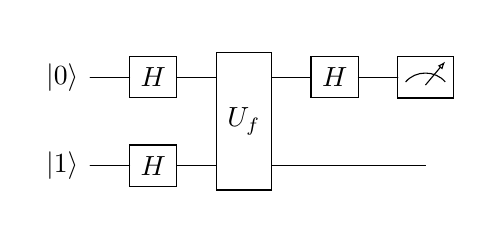
\begin{tikzpicture}
    \node[scale=1.0]{
    \begin{quantikz}[thin lines, transparent]
      \lstick{$\ket{0}$} & \gate{H} & \gate[2]{U_f} & \gate{H} & \meter{} \\
      \lstick{$\ket{1}$} & \gate{H} &               & \qw      & \qw
    \end{quantikz}};
  \end{tikzpicture}
  \caption{Deutsch's algorithm.
    The bottom qubit (ancilla) is initialized to $\ket{1}$; after $H$ it becomes $\ket{-}$, enabling phase kickback.
    The top qubit carries the answer.
  }
\end{figure}

After $H\otimes H$: $\displaystyle \ket{+}\ket{-}=\frac{1}{\sqrt{2}}(\ket{0}+\ket{1})\otimes\frac{1}{\sqrt{2}}(\ket{0}-\ket{1})$

After $U_f$ (phase kickback): $\displaystyle \frac{1}{\sqrt{2}}((-1)^{f(0)}\ket{0}+(-1)^{f(1)}\ket{1})\ket{-}$

Factor out $(-1)^{f(0)}$:
\begin{equation*}
  (-1)^{f(0)}\cdot\frac{1}{\sqrt{2}}(\ket{0}+(-1)^{f(0)\oplus f(1)}\ket{1})\ket{-}
\end{equation*}

If $f$ constant: $f(0)\oplus f(1)=0$, first register is $\ket{+}$.\\
If $f$ balanced: $f(0)\oplus f(1)=1$, first register is $\ket{-}$.

After $H$ on first register: $\ket{0}$ (constant) or $\ket{1}$ (balanced).

Measuring gives a \textbf{certain} answer in a single oracle call.

\begin{note}
  The key insight is that the answer to a \emph{global} property ($f(0)=f(1)$?) is encoded in the \emph{relative phase} between $\ket{0}$ and $\ket{1}$, which the final $H$ converts into a measurable bit.
\end{note}

\begin{lstlisting}
# input:  oracle $\gm{U_f}$ for unknown $\gm{f:\{0,1\}\to\{0,1\}}$
# output: "constant" if $\gm{f(0)=f(1)}$, "balanced" otherwise

deutsch($U_f$):
    # Prepare the two-qubit register.
    # The ancilla starts at $\gm{\ket{1}}$ so that H turns it into $\gm{\ket{-}}$,
    # enabling phase kickback when the oracle runs.
    $q_0$ = $\ket{0}$        # data qubit
    $q_1$ = $\ket{1}$        # ancilla (phase kickback target)

    H($q_0$,$q_1$)     # $\gm{H\ket{01} \to \ket{+}\ket{-}}$

    $U_f$($q_0$,$q_1$)
    # After this: $\gm{q_0}$ holds $\displaystyle \gm{\frac{1}{\sqrt{2}}((-1)^{f(0)}\ket{0} + (-1)^{f(1)}\ket{1})}$.
    # The oracle wrote $\gm{f}$ into the phase of $\gm{q_0}$,
    # leaving $\gm{q_1 = \ket{-}}$ unchanged.

    apply $H$ to $q_0$
    # H converts the phase difference into a deterministic bit:
    #   if $\gm{f(0) = f(1)}$ (constant) -> $\gm{q_0 = \ket{0}}$
    #   if $\gm{f(0) \neq f(1)}$ (balanced) -> $\gm{q_0 = \ket{1}}$

    result = measure($q_0$)

    if result == 0:
        return "constant"
    else:
        return "balanced"
\end{lstlisting}


\begin{exercise*}[Effect of a two-qubit circuit]
  The circuit below acts on two qubits (top wire first qubit, bottom wire second qubit), and $f$ is defined as $f(0)=1$, $f(1)=0$:
  \begin{center}
    \begin{quantikz}[thin lines, transparent, slice all, slice style=gray]
  & \gate{H} & \ctrl{1} & \gate{H} & \\
  & \gate{H} & \gate{U_f} & \gate{H} &
\end{quantikz}

  \end{center}
  Describe the effect on states $\ket{00}$ and $\ket{11}$.

  \textcolor{orange!140}{\rule{\textwidth}{1.5pt}}

  We remember that $U_f\ket{x}\ket{y}=\ket{x}\ket{y\oplus f(x)}$.

  \textbf{Case $\ket{\psi}=\ket{00}$.}
  After $H\otimes H$:
  \begin{equation*}
    \ket{\psi_1} = \frac{\ket{0}+\ket{1}}{\sqrt{2}}\otimes\frac{\ket{0}+\ket{1}}{\sqrt{2}}
    = \frac{\ket{00}+\ket{01}+\ket{10}+\ket{11}}{2}.
  \end{equation*}
  After $U_f$ ($f(0)=1$, $f(1)=0$, so $\ket{00}\to\ket{01}$, $\ket{01}\to\ket{00}$, $\ket{10}\to\ket{10}$, $\ket{11}\to\ket{11}$):
  \begin{equation*}
    \ket{\psi_2} = \frac{\ket{01}+\ket{00}+\ket{10}+\ket{11}}{2}.
  \end{equation*}
  After $H\otimes H$ again, one can verify all cross-terms cancel except $\ket{00}$:
  \begin{equation*}
    \ket{\psi_3} = \ket{00}.
  \end{equation*}
  So the circuit has \textbf{no net effect} on $\ket{00}$.

  \textbf{Case $\ket{\psi}=\ket{11}$.}
  After $H\otimes H$:
  \begin{equation*}
    \ket{\psi_1} = \frac{\ket{0}-\ket{1}}{\sqrt{2}}\otimes\frac{\ket{0}-\ket{1}}{\sqrt{2}} = \ket{-}\otimes\ket{-}.
  \end{equation*}
  After $U_f$ and the second $H\otimes H$, a shortcut using linearity: write $\ket{\psi_2}=-\ket{+}\otimes\ket{-}$ (the second qubit maps $\ket{-}\to\ket{-}$ under $f$, while the phase of the first qubit flips due to $f$), so:
  \begin{equation*}
    \ket{\psi_3} = H(-\ket{+})\otimes H\ket{-} = -\ket{0}\otimes\ket{1} = -\ket{01}.
  \end{equation*}
  The output is $\ket{01}$ (up to a global phase of $-1$, which is unobservable).
\end{exercise*}

\section{Deutsch-Jozsa}

\textbf{Problem}: given $f:\{0,1\}^n\to\{0,1\}$ promised to be either constant or balanced (exactly half the inputs map to 1), determine which.

Classically: worst case $2^{n-1}+1$ queries; randomized with high probability $O(1)$ queries, but never with certainty in fewer than $\Theta(2^n)$.
The Deutsch-Jozsa algorithm: \textbf{1 query}, deterministic.

\begin{figure}[H]
  \centering
  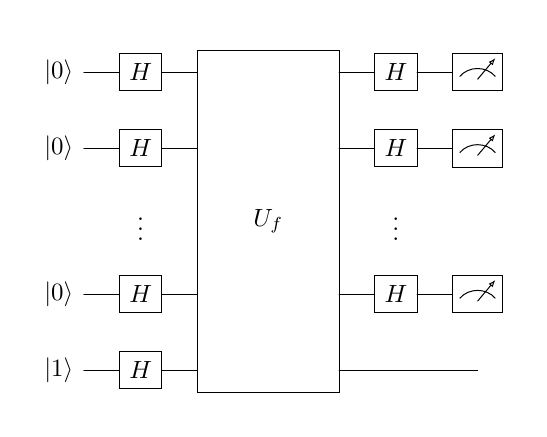
\begin{tikzpicture}
    \node[scale=0.9]{
    \begin{quantikz}[thin lines, transparent]
      \lstick{$\ket{0}$} & \gate{H} & \gate[5][2cm]{U_f} & \gate{H} & \meter{} \\
      \lstick{$\ket{0}$} & \gate{H} &                    & \gate{H} & \meter{} \\
      \setwiretype{n}    & \vdots   &                    & \vdots   &          \\
      \lstick{$\ket{0}$} & \gate{H} &                    & \gate{H} & \meter{} \\
      \lstick{$\ket{1}$} & \gate{H} &                    &          &
    \end{quantikz}};
  \end{tikzpicture}
  \caption{Deutsch-Jozsa circuit for $n$ data qubits plus one ancilla.
    Measure all $n$ data qubits: all-zeros $\Rightarrow$ constant; anything else $\Rightarrow$ balanced.
  }
\end{figure}

Use $n+1$ qubits initialized to $\ket{0}^{\otimes n}\ket{1}$.
Apply $H^{\otimes(n+1)}$, then $U_f$, then $H^{\otimes n}$ to the first $n$ qubits, then measure them.

\begin{lstlisting}
# input:  oracle $\gm{U_f}$ for $\gm{f:\{0,1\}^n\to\{0,1\}}$
# output: "constant" or "balanced"

deutsch_jozsa($U_f$,$n$):
    q = $\ket{0}^{\otimes n}$    # $\gm{n}$-qubit data register
    a = $\ket{1}$    # ancilla qubit for phase kickback

    $H^{\otimes n}$(q)  # uniform superposition: $\displaystyle \gm{\frac{1}{\sqrt{2^n}}\sum_x \ket{x}}$
    $H$(a)  # a $\gm{\to \ket{-}}$

    $U_f$(q,a)
    # Phase kickback: state becomes $\displaystyle \gm{\frac{1}{\sqrt{2^n}}\sum_x (-1)^{f(x)}\ket{x}\ket{-}}$
    # The sign of each $\gm{\ket{x}}$ encodes $\gm{f(x)}$; a is untouched.

    $H^{\otimes n}$(q)
    # Interference: amplitude of $\gm{\ket{0}^n}$ is $\displaystyle \gm{\frac{1}{2^n}\sum_x (-1)^{f(x)}}$
    #   constant $\gm{f}$: all signs equal, sum = +- 1 -> $\gm{\ket{0}^n}$ with prob 1
    #   balanced $\gm{f}$: half +1, half -1, sum = 0  -> $\gm{\ket{0}^n}$ with prob 0

    result = measure(q)

    if result == $0^n$:
        return "constant"
    else:
        return "balanced"
\end{lstlisting}

After the first $H^{\otimes(n+1)}$ the state is $\displaystyle \frac{1}{\sqrt{2^n}}\sum_{x\in\{0,1\}^n}\ket{x}\ket{-}$.

After $U_f$ (phase kickback): $\displaystyle \frac{1}{\sqrt{2^n}}\sum_x(-1)^{f(x)}\ket{x}\ket{-}$.

After $H^{\otimes n}$ on the data register, using $\displaystyle H^{\otimes n}\ket{x}=\frac{1}{\sqrt{2^n}}\sum_z(-1)^{x\cdot z}\ket{z}$:
\begin{equation*}
  \sum_{z\in\{0,1\}^n}\left[\frac{1}{2^n}\sum_{x}(-1)^{f(x)+x\cdot z}\right]\ket{z}
\end{equation*}

The amplitude of $\ket{0}^{\otimes n}$ is $\displaystyle \frac{1}{2^n}\sum_x(-1)^{f(x)}$.
\begin{itemize}
  \item $f$ constant $\Rightarrow$ all $(-1)^{f(x)}$ equal $\pm1$ $\Rightarrow$ sum $=\pm1$ $\Rightarrow$ probability 1 of measuring $\ket{0}^{\otimes n}$;
  \item $f$ balanced $\Rightarrow$ half are $+1$, half $-1$ $\Rightarrow$ sum $=0$ $\Rightarrow$ probability 0 of measuring $\ket{0}^{\otimes n}$.
\end{itemize}

One measurement suffices to determine the answer with certainty.

\begin{note}
  The Deutsch-Jozsa algorithm is somewhat artificial (the constant-or-balanced promise is strong), but it cleanly demonstrates an exponential separation and introduces all the techniques (phase kickback + Hadamard interference) used in more practical algorithms.
\end{note}

\section{Simon}

Simon's algorithm (1994) was historically important because it gave the first exponential quantum speedup for a \emph{structured} problem, and directly inspired Shor's factoring algorithm.

\textbf{Problem}: given $f:\{0,1\}^n\to\{0,1\}^n$ promised to satisfy $f(x)=f(y)$ iff $x\oplus y\in\{0^n,s\}$ for some fixed hidden string $s\in\{0,1\}^n$, find $s$.

\begin{itemize}
  \item If $s=0^n$: $f$ is injective.
  \item If $s\neq0^n$: $f$ is exactly 2-to-1; every value is achieved by exactly the pair $\{x,\,x\oplus s\}$.
\end{itemize}

Classically, finding $s$ requires $\Omega(\sqrt{2^n})$ queries (birthday-paradox argument).
Simon's algorithm finds $s$ in $O(n)$ queries.

\begin{lstlisting}
# input:  oracle $\gm{U_f}$ for $\gm{f:\{0,1\}^n\to\{0,1\}^n}$, promised to hide secret s
# output: the hidden string s $\gm{\in \{0,1\}^n}$

simon($U_f$, n):
    system = []      # will collect constraint vectors z with zs = 0

    # repeat until n-1 linearly independent vectors in system
    while system.size() < n-1:

        q = $\ket{0}^{\otimes n}$    # data register
        r = $\ket{0}^{\otimes n}$    # output register

        $H^{\otimes n}$(q)
        # q is now the uniform superposition $\displaystyle \gm{\frac{1}{\sqrt{2^n}}\sum_x \ket{x}}$

        $U_f$(q,r)
        # joint state: $\displaystyle \gm{\frac{1}{\sqrt{2^n}}\sum_x \ket{x}\ket{f(x)}}$

        measure(r)
        # we observe some value $\gm{f(x_0)}$; q collapses to
        #       $\displaystyle \gm{\frac{1}{\sqrt{2}}(\ket{x_0} + \ket{x_0 \oplus s})}$
        # (the two pre-images that give the same output
        # collapse together)

        $H^{\otimes n}$(q)
        # amplitudes cancel for every z with zs = 1 (mod 2),
        # so only strings z satisfying zs=0 have nonzero amplitude.

        z = measure(q)    # always a valid constraint zs=0
        system.append(z)

    # Solve system $\gm{\{\text{z}^{i} \text{s} = 0\}}$ with Gaussian elimination and recover s
    s = solve(system)
    return s
\end{lstlisting}

After step 4, $H^{\otimes n}$ on $\displaystyle\frac{\ket{x_0}+\ket{x_0\oplus s}}{\sqrt{2}}$ yields:
\begin{equation*}
  \frac{1}{\sqrt{2^{n+1}}}\sum_z[(-1)^{z\cdot x_0}+(-1)^{z\cdot(x_0\oplus s)}]\ket{z}
  =\frac{1}{\sqrt{2^{n+1}}}\sum_z(-1)^{z\cdot x_0}[1+(-1)^{z\cdot s}]\ket{z}
\end{equation*}
The amplitude of $\ket{z}$ is zero unless $z\cdot s=0\pmod2$.
So the measurement always yields some $z$ satisfying $\mathbf{z\cdot s=0}$.

After $O(n)$ rounds we have $n-1$ linearly independent equations $z^{(i)}\cdot s=0$, from which $s$ is determined by system solving via Gaussian elimination over $\mathbb{F}_2$, leaving with total complexity: $O(n)$.

\begin{figure}[H]
  \centering
  \begin{quantikz}[thin lines, transparent]
    \lstick{$\ket{0}^{\otimes n}$} & \gate{H^{\otimes n}} & \gate[2][2cm]{U_f}\gateinput{$\ket{x}$}\gateoutput{$\ket{x}$} & \gate{H^{\otimes n}} & \meter{} & \rstick{$\small y \cdot s = 0 \bmod 2$} \\
    \lstick{$\ket{0}^{\otimes n}$} & & \gateinput{$\ket{0}$}\gateoutput{$\ket{f(x)}$} & \meter{} & & \rstick{$\displaystyle \frac{\ket{x} + \ket{x \xor s}}{\sqrt{2}}$}
  \end{quantikz}
  \caption{Simon circuit.}
\end{figure}

\begin{note}
  Simon's problem is about the \emph{hidden subgroup} $\{0,s\}$ of $(\mathbb{Z}_2)^n$.
  Shor's algorithm (next section) solves the analogous problem for $\mathbb{Z}_N$, where the \quoted{hidden subgroup} is $\{0,r,2r,\ldots\}$ generated by the order $r$ of an element.
  The Quantum Fourier Transform is the generalization of $H^{\otimes n}$ that unlocks this.
\end{note}

\section{Quantum Fourier Transform}

\begin{definition*}[QFT]
  The \emph{Quantum Fourier Transform} on $\mathbb{Z}_N$ is:
  \begin{equation*}
    \mathrm{QFT}_N\ket{j}=\frac{1}{\sqrt{N}}\sum_{k=0}^{N-1}\w^{jk}\ket{k}
  \end{equation*}
  where
  \begin{itemize}
    \item $N = 2^n$ is the number of states
    \item $\w = e^{\frac{2 \pi i}{N}}$ is the $N$-th root of unity
  \end{itemize}
  and $j,k$ are respectively the input and output states.
\end{definition*}

It is the quantum analogue of the classical DFT, but acting on amplitudes.
Key properties:
\begin{itemize}
  \item Unitary (preserves norms);
  \item Implements the same linear map as the DFT but in $O(n^2)$ gates, exponentially fewer than the classical FFT's $O(n\cdot2^n)$ operations.
\end{itemize}

\subsection{Product Representation}

Writing $j=j_1 2^{n-1}+\cdots+j_n 2^0$ in binary, the QFT has the elegant product form:
\begin{equation*}
  \mathrm{QFT}_N\ket{j_1\cdots j_n}=\frac{1}{\sqrt{N}} \bigotimes_{t=1}^{n}\!\left(\ket{0}+e^{2\pi i\,0.j_t j_{t+1}\cdots j_n}\ket{1}\right)
\end{equation*}
where
\begin{equation*}
  0.j_t \cdots j_n=\sum_t^n \frac{j_t}{2^{n-t+1}}
\end{equation*}
is a binary fraction (\eg, $0.j_1 \cdots j_n = \frac{j_1}{2}+\frac{j_2}{4}+\cdots+\frac{j_n}{2^n}$).

Each output qubit is in an independent superposition; the circuit can be built qubit by qubit.

\subsection{Circuit}

The QFT circuit uses $n$ Hadamard gates and $\displaystyle \frac{n(n-1)}{2}$ controlled rotation gates
\begin{equation*}
  R_k=\text{diag}(1,e^{2\pi i/2^k}),
\end{equation*}
followed by a reversal of qubit order (SWAP gates).
Total: $O(n^2)$ gates.

For $n=3$ qubits the circuit is:
\begin{figure}[H]
  \centering
  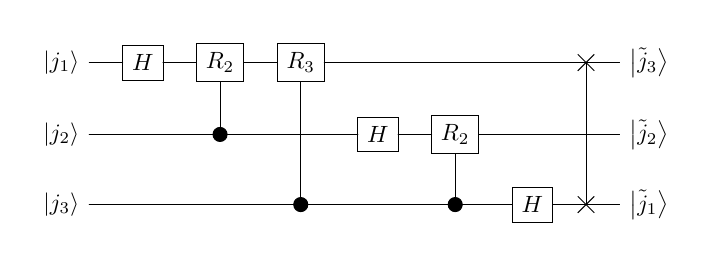
\begin{tikzpicture}
    \node[scale=0.85]{
    \begin{quantikz}[thin lines, transparent]
      \lstick{$\ket{j_1}$} & \gate{H} & \gate{R_2} & \gate{R_3} & \qw        & \qw        & \qw      & \swap{2}  & \qw \rstick{$\ket{\tilde{j}_3}$} \\
      \lstick{$\ket{j_2}$} & \qw      & \ctrl{-1}  & \qw        & \gate{H}   & \gate{R_2} & \qw      & \qw       & \qw \rstick{$\ket{\tilde{j}_2}$} \\
      \lstick{$\ket{j_3}$} & \qw      & \qw        & \ctrl{-2}  & \qw        & \ctrl{-1}  & \gate{H} & \targX{}  & \qw \rstick{$\ket{\tilde{j}_1}$}
    \end{quantikz}};
  \end{tikzpicture}
  \caption{QFT circuit for $n=3$.
    Each qubit receives one Hadamard and controlled-$R_k$ phases from all lower qubits.
    The final SWAPs reverse the qubit order (the product representation outputs bits in reverse significance).
    Gate $R_k=\mathrm{diag}(1,e^{2\pi i/2^k})$.
  }
\end{figure}

For a general $n$ is instead:
\begin{figure}[H]
  \centering
  \begin{adjustbox}{max width=\textwidth}
    \begin{quantikz}[thin lines, transparent]
      \lstick{$\ket{j_1}$} & \gate{H} & \gate{R_2} & \gate{R_3} & \ \dots \ & \gate{R_n} & & & & & & & & & \ \dots \ & & \rstick{$\ket{0} + e^{2 \pi i 0.j_1 j_2 \dots j_n} \ket{1}$} \\
      \lstick{$\ket{j_2}$} & & \ctrl{-1} & & & & \gate{H} & \gate{R_2} & \ \dots \ & \gate{R_{n-1}} & & & & & \ \dots \ & & \rstick{$\ket{0} + e^{2 \pi i 0.j_2 \dots j_n} \ket{1}$} \\
      \lstick{$\ket{j_3}$} & & & \ctrl{-2} & & & & \ctrl{-1} & & & \gate{H} & \gate{R_2} & \ \dots \ & \gate{R_{n-2}} & \ \dots \ & & \rstick{$\ket{0} + e^{2 \pi i 0.j_3 \dots j_n} \ket{1}$} \\
      \setwiretype{n}\lstick{\vdots} & & & & & & & & \vdots & & & & & & & & & \rstick{\vdots} \\
      \lstick{$\ket{j_n}$} & & & & & \ctrl{-4} & & & & \ctrl{-3} & & & & \ctrl{-2} & \ \dots \ & \gate{H} & \rstick{$\ket{0} + e^{2 \pi i 0.j_n} \ket{1}$} \\
    \end{quantikz}
  \end{adjustbox}
  \caption{General circuit for size $n$.}
\end{figure}

\begin{note}
  In the above figure, the last SWAP among all states has been omitted, because it's common practice to not apply the SWAP gate inside the circuit to not mess with the noise.
  Instead the outputs are read/used backwards, and in this way they're still able to use them in the correct order.
\end{note}

\begin{lstlisting}
# input:  n-qubit register holding $\gm{\ket{j_1 j_2 \cdots j_n}}$
# output: same register holding $\gm{\mathrm{QFT}_N\ket{j_1 \cdots j_n}}$
# gates used: $\gm{H}$ (Hadamard), $\gm{R_k}$ (controlled phase $\gm{e^{2\pi i / 2^k}}$), SWAP

QFT(n):
    for t in range(1,n):
        $H$(t)
        # qubit t now has factor $\gm{(\ket{0} + e^{2\pi i\, 0.j_t}\ket{1})}$

        for k in range(2,n-t+1):
            $R_k$(t+k-1,t)
            # each controlled-$\gm{R_k}$ appends one more binary
            # digit to the phase:
            # after all k, qubit t holds $\gm{(\ket{0} + e^{2\pi i\, 0.j_t j_{t+1} \cdots j_n}\ket{1})}$

    # The product representation is now built qubit by qubit,
    # but the bit order is reversed; fixed with SWAPs
    for i in range(1, $\lfloor n/2 \rfloor$):
        SWAP(i,n-i+1)

# The inverse circuit and replace each $\gm{R_k}$ with $\gm{R_k^\dagger}$,
# i.e. negate all phase angles
QFT$^\dagger$(n):
    for i in range(1, $\lfloor n/2 \rfloor$):
        SWAP(i,n-i+1)

    for t in range(n,1,-1):
        for k in range(n-t+1,2,-1):
            $R_k^\dagger$(t+k-1,t)  # phase $\gm{-e^{2\pi i / 2^k}}$
        $H$(t)
\end{lstlisting}

The inverseQFT is used in QPE and Shor's algorithm.

\begin{example*}[QFT on 2 qubits ($N=4$)]
  Apply to $\ket{j_1 j_2}$:
  \begin{enumerate}
    \item $H$ on $q_1$: $\frac{1}{\sqrt{2}}(\ket{0}+e^{2\pi i\,0.j_1}\ket{1})\ket{j_2}$;
    \item Controlled-$R_2$ with control $q_2$: adds phase $e^{2\pi i j_2/4}$ to $q_1$'s $\ket{1}$ component, giving $\frac{1}{\sqrt{2}}(\ket{0}+e^{2\pi i\,0.j_1 j_2}\ket{1})\ket{j_2}$;
    \item $H$ on $q_2$: $\ket{q_2}\to\frac{1}{\sqrt{2}}(\ket{0}+e^{2\pi i\,0.j_2}\ket{1})$;
    \item SWAP $q_1\leftrightarrow q_2$.
  \end{enumerate}
  Result: $\frac{1}{2}(\ket{0}+e^{i\pi j_2}\ket{1})\otimes(\ket{0}+e^{i\pi j_1+i\pi j_2/2}\ket{1})$, which is indeed $\frac{1}{2}\sum_{k=0}^3 e^{2\pi ijk/4}\ket{k}$.
\end{example*}

\subsection{Quantum Phase Estimation}

\textbf{Quantum Phase Estimation} (QPE) is one of the most important subroutines in quantum computing.
Given a unitary $U$ and an eigenstate $\ket{u}$ with $U\ket{u}=e^{2\pi i\phi}\ket{u}$, estimate $\phi$ to $n$ bits of precision.

\textbf{Circuit}: use two registers.
First register: $t$ ancilla qubits initialized to $\ket{0}^{\otimes t}$.
Second register: the eigenstate $\ket{u}$.

\begin{lstlisting}
# input:  unitary $\gm{U}$, eigenstate $\gm{\ket{u}}$ with $\gm{U\ket{u} = e^{2\pi i\phi}\ket{u}}$,
#         precision t (number of phase register qubits)
# output: $\gm{\tilde{\phi}}$, an estimate of $\gm{\phi}$ accurate to $\gm{2^{-t}}$ with high probability

QPE($U$, $\ket{u}$, t):
    p = $\ket{0}^{\otimes t}$    # phase register (will hold the estimate)
    e = $\ket{u}$   # eigenstate register

    $H^{\otimes t}$(p)
    # p is now the uniform superposition $\displaystyle \gm{\frac{1}{\sqrt{2^t}}\sum_{k=0}^{2^t-1}\ket{k}}$

    for j in range(0,t-1):
        $U^{2^j}$(p[j],e)
        # Qubit j of p picks up phase $\gm{e^{2\pi i \phi \cdot 2^j}}$ when it is $\gm{\ket{1}}$.
        # After all controlled powers, p holds
        #     $\displaystyle \gm{\frac{1}{\sqrt{2^t}}\sum_k e^{2\pi i \phi k}\ket{k}}$
        # this is QFT($\gm{\phi \cdot 2^t}$).

    QFT$^\dagger$(p)
    # The inverse QFT maps the phase-encoded state back to a
    # computational basis state peaked sharply at the integer
    # nearest to $\gm{\phi \cdot 2^t}$.

    $\tilde{m}$ = measure(p)      # integer in $\gm{\{0, \ldots, 2^t - 1\}}$
    return $\tilde{\phi}$ = $\displaystyle \frac{\tilde{m}}{2^t}$
    # With $\gm{\geq 1 - \e}$ probability, $\gm{|\tilde{\phi} - \phi| \leq 2^{-t}}$.
\end{lstlisting}

After step 2, the first register holds $\displaystyle \frac{1}{\sqrt{2^t}}\sum_{k=0}^{2^t-1}e^{2\pi i\phi k}\ket{k}$, which is the QFT of a state peaked at $\phi\cdot 2^t$.
The inverse QFT concentrates amplitude on the integer nearest $\phi\cdot 2^t$.
With $\displaystyle t=n+\lceil\log(2+\frac{1}{2\varepsilon})\rceil$ qubits, we get $|\tilde\phi-\phi|<2^{-n}$ with probability $\ge1-\varepsilon$.

\section{Shor}

Shor (1994) showed that integer factoring can be done in polynomial time on a quantum computer, threatening essentially all public-key cryptography in use today (RSA, DH, elliptic curve).

Given $N$, choose $a$ with $\gcd(a,N)=1$ (otherwise we've already found a factor).
The \textbf{order} of $a$ modulo $N$ is the smallest $r>0$ with $a^r\equiv1\pmod N$.

\textbf{Claim}: if $r$ is even and $a^{r/2}\not\equiv-1\pmod N$, then at least one of $\gcd(a^{r/2}\pm1,N)$ is a nontrivial factor.

\textbf{Proof sketch}: $a^r-1\equiv0$ so $(a^{r/2}-1)(a^{r/2}+1)\equiv0\pmod N$. Under the given conditions neither factor is 0 mod $N$, so $N$ must split between them --- Euclid's algorithm finds the factors.

It can be shown that for random $a$, the probability of $r$ being even and $a^{r/2}\not\equiv-1\pmod N$ is at least $1/2$ (and much higher in practice).

\begin{lstlisting}
# input:  composite integer N
# output: a nontrivial factor p of N

shor(N):
    # Classical pre-processing
    if N is even:
        return 2   # trivial case

    # Pick a random base and check if we got lucky
    a = randint(2,N-1)
    g = gcd(a, N)
    if g > 1:
        return g    # found a factor without any quantum step

    # Quantum order-finding
    # The order r is the smallest positive r with $\gm{a^r \equiv 1 \pmod{N}}$.
    # We find it by running QPE on the unitary $\gm{U_a: \ket{x} \mapsto \ket{ax \bmod N}}$.
    r = quantum_order_finding(a, N)
    # QPE gives a random s/r -> continued fractions recovers r.

    if r is odd or $a^{r/2} \equiv -1 \pmod{N}$:
        # Bad a choice: the reduction to factoring fails.
        # This happens with probability $\gm{\leq 1/2}$; retry with new a
        return shor(N)      # restart

    # Now $\gm{(a^{r/2} - 1)(a^{r/2} + 1) \equiv 0 \pmod{N}}$,
    # but neither factor is 0 mod N, so N must split
    p = gcd($a^{r/2} - 1$, N)
    q = gcd($a^{r/2} + 1$, N)

    for candidate in [p, q]:
        if 1 < candidate < N:
            return candidate  # nontrivial factor found

    # p,q were 0 or multiple of N
    return shor(N)


quantum_order_finding(a, N):
    # Use QPE on $\gm{U_a:\ket{x}\mapsto\ket{ax \bmod N}}$ with input state $\gm{\ket{1}}$.
    # $\displaystyle \gm{\ket{1} = \frac{1}{\sqrt{r}}\sum_{s=0}^{r-1}\ket{u_s}}$, a superposition of
    # all eigenstates, so QPE returns a random eigenphase s/r.
    $\tilde{\phi}$ = QPE($U_a$, $\ket{1}$, t=2n+3)   # t bits of precision

    # Continued fraction expansion of $\gm{\tilde{\phi}}$ gives the fraction s/r
    # in lowest terms; the denominator is a candidate for r.
    r = denominator(continued_fraction($\tilde{\phi}$))
    if $a^r \equiv 1 \pmod{N}$:
        return r
    else:
        # retry (rare, O(1) times expected)
        return quantum_order_finding(a, N)
\end{lstlisting}

\begin{example*}[Factoring 15]
  Let $N=15$, $a=7$.
  The order of 7 mod 15:
  \begin{equation*}
    7^1=7,\ 7^2=49 \equiv 4,\ 7^3 \equiv 28 \equiv 13,\ 7^4 \equiv 91 \equiv 1,
  \end{equation*}
  so $r=4$.
  
  Check: $r=4$ is even; $7^2=49\equiv4\not\equiv-1\equiv14\pmod{15}$.
  $\gcd(7^2-1,15)=\gcd(48,15)=\gcd(3,15)=3$. \quad Factor found: \textbf{3}.
  $\gcd(7^2+1,15)=\gcd(50,15)=\gcd(5,15)=5$. \quad Factor found: \textbf{5}.
  Indeed, $15=3\times5$.
\end{example*}

The quantum order-finding circuit uses $O(n)$ qubits and $O(n^3)$ gates (where $N<2^n$), giving an overall algorithm that is polynomial in $\log N$.
The best classical algorithms run in $\exp(O(n^{1/3}\log^{2/3}n))$ time (subexponential but not polynomial).

\begin{note}
  \textbf{Threat to cryptography}: RSA-2048 has $N\approx2^{2048}$, requiring $n\approx2048$.
  A fault-tolerant quantum computer would need of order millions of physical qubits to factor it; this is beyond current hardware (which has $O(10^3)$ qubits with high error rates) but motivates urgent migration to post-quantum cryptography.
\end{note}

\section{Grover}

\textbf{Problem}: given an oracle for a function $f:\{0,1\}^n\to\{0,1\}$ with exactly one \emph{marked} element $\omega$ (\ie, $f(\omega)=1$ and $f(x)=0$ for $x\neq\omega$), find $\omega$.

Classically: $\Theta(N)$ queries in the worst case ($N=2^n$).
Grover's algorithm (1996): $O(\sqrt{N})$ queries.
This is \textbf{optimal}: no quantum algorithm can do better.

The algorithm starts with the uniform superposition $\ket{s}=H^{\otimes n}\ket{0}^{\otimes n}=\frac{1}{\sqrt{N}}\sum_x\ket{x}$.

Each \textbf{Grover iteration} $G=D\cdot O$ applies:
\begin{enumerate}
  \item \textbf{Oracle $O$}: $O\ket{x}=(-1)^{f(x)}\ket{x}$ (phase
    flip the marked state).
  \item \textbf{Diffusion $D$}: $D=2\ket{s}\bra{s}-I$ (inversion
    about the mean).
\end{enumerate}

The diffusion operator $D$ maps each amplitude $a_x\mapsto2\bar a-a_x$ where $\bar a=\frac{1}{N}\sum_x a_x$ is the mean.
This \emph{amplifies} amplitudes above the mean and suppresses those below; after the oracle has made the marked amplitude negative, the diffusion step boosts it towards 1.

Let $\ket{\omega}$ be the marked state and $\ket{\omega^\perp}=\frac{1}{\sqrt{N-1}}\sum_{x\neq\omega}\ket{x}$ the uniform superposition over non-solutions.
The initial state is:
\begin{equation*}
  \ket{s}=\frac{1}{\sqrt{N}}\ket{\omega}+\sqrt{\frac{N-1}{N}}\ket{\omega^\perp}=\sin\theta\ket{\omega}+\cos\theta\ket{\omega^\perp}
\end{equation*}
where $\sin\theta=\frac{1}{\sqrt{N}}$.

The oracle $O$ reflects through $\ket{\omega^\perp}$ (negates the $\ket\omega$ component); the diffusion $D$ reflects through $\ket{s}$.
Two reflections around axes separated by angle $\theta$ compose to a rotation by $2\theta$, so each Grover iteration $G = D\cdot O$ rotates the state by $2\theta$ toward $\ket\omega$.

\begin{figure}[H]
  \centering
  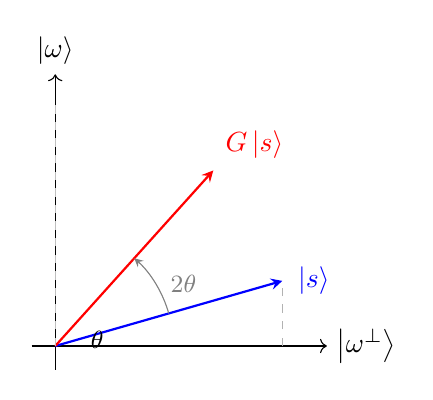
\begin{tikzpicture}[scale=3.0]
    \draw[->] (-0.1,0) -- (1.15,0) node[right] {$\ket{\omega^\perp}$};
    \draw[->] (0,-0.1) -- (0,1.15) node[above] {$\ket{\omega}$};
    % initial state |s> at angle theta from x-axis
    \def\thdeg{16}
    \draw[thick,blue,-stealth] (0,0) -- ({cos(\thdeg)},{sin(\thdeg)})
      node[right=2pt] {$\ket{s}$};
    % after one iteration: angle (3*theta)
    \def\tkdeg{48}
    \draw[thick,red,-stealth] (0,0) -- ({cos(\tkdeg)},{sin(\tkdeg)})
      node[above right=1pt] {$G\ket{s}$};
    % arc
    \draw[-stealth,gray] ({0.5*cos(\thdeg)},{0.5*sin(\thdeg)})
      arc[start angle=\thdeg, end angle=\tkdeg, radius=0.5]
      node[midway,right=2pt]{\small$2\theta$};
    % theta label
    \draw[dashed,gray!60] ({cos(\thdeg)},0) -- ({cos(\thdeg)},{sin(\thdeg)});
    \node at ({0.18*cos(\thdeg/2)},{0.18*sin(\thdeg/2)}) {\small$\theta$};
    % target |omega>
    \draw[dashed,gray!50] (0,0) -- (0,1.05);
  \end{tikzpicture}
  \caption{One Grover iteration rotates the state by $2\theta$ in the two-dimensional plane spanned by $\ket{\omega}$ and $\ket{\omega^\perp}$.
    Starting from the small angle $\theta\approx1/\sqrt{N}$, after $k^*\approx\frac\pi4\sqrt{N}$ rotations the state is close to $\ket{\omega}$ (the vertical axis) and measurement succeeds with high probability.
  }
\end{figure}

Each Grover iteration rotates the state by $2\theta$ in the $(\ket{\omega},\ket{\omega^\perp})$ plane.
After $k$ iterations the angle from $\ket{\omega^\perp}$ is $(2k+1)\theta$.
We want this near $\pi/2$, so the optimal number of iterations is:
\begin{equation*}
  k^*=\left\lfloor\frac{\pi}{4\theta}\right\rfloor\approx\frac{\pi}{4}\sqrt{N}
\end{equation*}
After $k^*$ iterations, $|\braket{\omega}{\psi}|^2\approx1$, and measuring gives $\omega$ with high probability.

\begin{example*}[Grover with $N=4$, $\omega=\ket{11}$]
  $\theta=\pi/6$ (since $\sin\theta=1/2$), so $k^*=1$ exactly.
  
  Start: $\ket{s}=\frac{1}{2}(\ket{00}+\ket{01}+\ket{10}+\ket{11})$.
  
  After oracle $O$: $\frac{1}{2}(\ket{00}+\ket{01}+\ket{10}-\ket{11})$.
  Mean amplitude: $\bar a=\frac{1}{4}(1+1+1-1)=\frac{1}{2}$.
  
  After diffusion ($a_x\to 2\bar a - a_x$): non-marked amplitudes become $2\cdot\frac12-\frac12=\frac12\to 0$; marked amplitude becomes $2\cdot\frac12-(-\frac12)=1$.
  
  Result: $\ket{11}$ with probability 1 after a single iteration.
\end{example*}

\begin{lstlisting}
# input:  oracle $\gm{O_f}$ with $\gm{O_f\ket{x} = (-1)^{f(x)}\ket{x}}$, search space size $\gm{N = 2^n}$
# output: the marked element $\gm{\omega}$ with $\gm{f(\omega) = 1}$

grover($O_f$, n):
    q = $\ket{0}^{\otimes n}$

    $H^{\otimes n}$(q)
    # q = $\displaystyle \gm{\ket{s} = \frac{1}{\sqrt{N}}\sum_x \ket{x}}$  (uniform superposition)

    # Compute optimal number of iterations: $\displaystyle \gm{k^* \approx \frac{\pi}{4}\sqrt{N}}$
    # (More precisely: $\displaystyle \gm{k^* = \lfloor \frac{\frac{\pi}{4}}{\arcsin(1/\sqrt{N})} \rfloor}$)
    $k^*$ = round($\displaystyle \frac{\pi}{4} \cdot \sqrt{N}$)

    loop $k^*$ times:

        # Oracle step: flip the phase of the marked state
        $O_f$(q)
        # $\gm{\ket{\omega}}$ picks up a -1 phase; all other amplitudes unchanged.
        # Geometrically: reflect through $\gm{\ket{\omega^\perp}}$.

        # Diffusion step: inversion about the mean
        $H^{\otimes n}$(q)
        phase flip on $\ket{0}^n$ only  # i.e. $\gm{2\ket{0}\bra{0} - I}$
        $H^{\otimes n}$(q)
        # Net effect: $\gm{a_x \mapsto 2\bar{a} - a_x}$ where $\gm{\bar{a}}$ is the mean amplitude.
        # Geometrically: reflect through $\gm{\ket{s}}$.
        # Combined with the oracle step: rotation by $\gm{2\theta}$ toward $\gm{\ket{\omega}}$.

    return measure(q)
    # After $\gm{k^*}$ iterations: $\gm{|\braket{\omega}{\mathbf{q}}|^2 \approx 1}$.
    # Wrong answer probability $\displaystyle \gm{\approx \sin^2(k^* \cdot 2\theta - \frac{\pi}{2}) \leq O(1/N)}$.
\end{lstlisting}

If there are $M$ marked elements (all with $f(x)=1$), the optimal number of iterations is $\approx\frac\pi4\sqrt{N/M}$, reducing to $\sqrt{N/M}$ queries total.

Grover's algorithm is \textbf{optimal}: any quantum algorithm for unstructured search needs $\Omega(\sqrt{N})$ queries.
The proof uses a \quoted{hybrid argument}: each query can change the success probability by at most $O(1/\sqrt{N})$ per step, so $\Omega(\sqrt{N})$ steps are needed.

\section{Quantum Complexity}

\begin{definition*}[BQP]
  \emph{Bounded-error Quantum Polynomial time} (BQP) is the class of decision problems solvable by a polynomial-size quantum circuit with error probability $\le1/3$ on every input.
\end{definition*}

\begin{center}
  \renewcommand{\arraystretch}{1.2}
  \begin{tabular}{l|l}
    \textbf{Containment} & \textbf{Meaning} \\
    \hline
    $\mathrm{P}\subseteq\mathrm{BPP}\subseteq\mathrm{BQP}$ & QC solves everything classical probabilistic does \\
    $\mathrm{BQP}\subseteq\mathrm{PSPACE}$ & QC is not all-powerful; it fits in polynomial space \\
    Factoring $\in$ BQP & Shor's algorithm (believed not in BPP) \\
    NP $\not\subseteq$ BQP (believed) & QC probably can't solve NP-hard problems \\
    $\mathrm{BQP}$ and NP incomparable\footnotemark & \\
  \end{tabular}
\end{center}
\footnotetext{conjectured}
\begin{note}
  A common misconception: \quoted{quantum computers can solve NP-complete problems}.
  Grover gives only a \emph{quadratic} speedup for unstructured search ($\sqrt{2^n}$ instead of $2^n$), which is still exponential in $n$.
  Factoring is \emph{not} believed to be NP-complete; it lives in a complexity class (probably) between P and NP.
\end{note}

\chapter{Quantum Key Distribution}

The security of classical public-key cryptography (RSA, Diffie-Hellman) rests on \emph{computational} hardness assumptions: we believe certain problems (factoring, discrete log) are hard for classical computers, but we have no proof.
Shor's algorithm shows that a sufficiently large quantum computer would break all of these.

\textbf{Quantum key distribution} (QKD) offers a fundamentally different security model: security based on the laws of physics, not on computational assumptions.
The eavesdropper can have unlimited computing power and it still cannot break a properly implemented QKD scheme.

\section{BB84 Protocol}

BB84 (Bennett and Brassard, 1984) is the first and most widely studied QKD protocol.

Two complementary bases for a single qubit:
\begin{itemize}
  \item \textbf{Rectilinear ($+$) basis}: $\ket{0}\leftrightarrow\text{bit }0$, $\ket{1}\leftrightarrow\text{bit }1$.
  \item \textbf{Diagonal ($\times$) basis}: $\ket{+}\leftrightarrow\text{bit }0$, $\ket{-}\leftrightarrow\text{bit }1$.
\end{itemize}

\begin{center}
  \renewcommand{\arraystretch}{1.3}
  \begin{tabular}{c|c|c}
    \textbf{Bit} & \textbf{$+$ basis} & \textbf{$\times$ basis} \\
    \hline
    0 & $\ket{0}$ & $\ket{+}$ \\
    1 & $\ket{1}$ & $\ket{-}$ \\
  \end{tabular}
\end{center}

The crucial property: measuring a $+$-basis state in the $\times$ basis gives a random result (50/50).
This is because $\ket{0}=\frac{\ket{+}+\ket{-}}{\sqrt{2}}$, so measurement in the $\times$ basis gives $\ket{+}$ (bit 0) or $\ket{-}$ (bit 1) with equal probability.

\begin{lstlisting}
# Participants: Alice (sender), Bob (receiver),
#     Eve (potential eavesdropper)
# Goal: establish a shared secret key of length l bits

BB84(l):

    # Quantum phase
    a,b,a2,b2 = [], [], [], []

    while len(a) >> l:

        # Alice side
        bit = rand(0,1) # picks a random bit
        basis = rand($+, \times$) # picks random basis
        q = encode(bit, basis)
        send(q,Bob)

        a.append(bit)
        b.append(basis)

        # Bob side
        basis2 = rand($+, \times$)
        q = receive()
        # measure received qubit in basis2
        result = measure(q,basis2)

        a2.append(result)
        b2.append(basis2)

    # Public channel (basis shifting)
    Alice publicly announce b
    Bob publicly announce b2
    sifted_key_A = [a[i] for i where b[i] = b2[i]]
    sifted_key_B = [a2[i] for i where b[i] = b2[i]]
    # Discard ~50% of bits where bases disagreed; keep the rest.
    # When bases agree, Bob's result = Alice's bit, 
    # thus no eavesdropping, because he measured in the
    # correct basis.

    # Error estimation
    sample random subset T of sifted key positions
    compare(sifted_key_A[T], sifted_key_B[T])
    QBER = (number of disagreements in T) / len(T)

    if QBER > 0.11:    # threshold ~11%
        abort()
        # Too many errors: either Eve is present
        # or channel noise is too high.
        # Any intercept-resend attack by Eve produces
        # QBER $\gm{\approx}$ 25\%.

    # Error correction + Privacy amplification
    remove sample positions T from both sifted keys
    reconciled_key = error_correct(sifted_key_A, sifted_key_B)
    # Error correction fixes the remaining ~QBER fraction of
    # mismatches, at the cost of leaking some information to Eve.

    final_key = privacy_amplify(reconciled_key, QBER)
    # Universal hashing compresses the key by the amount
    # of information Eve could have learned, making her
    # knowledge negligible.
    # Output length l $\gm{\approx}$ len(reconciled_key)*(1 - H(QBER))
    # where H is the binary entropy function.

    return final_key    # shared secret
\end{lstlisting}

\begin{question*}[Why Eavesdropping Is Detectable?]
  Suppose Eve intercepts every qubit, measures in a random basis, and resends.
  She guesses the right basis half the time.
  When she guesses wrong:
  \begin{itemize}
    \item Her measurement gives a random result (no information);
    \item She resends in the wrong basis; Bob, measuring in Alice's (correct) basis, now gets a random result;
    \item This introduces errors: when Alice and Bob both used the $+$ basis, Eve's interception causes Bob to get the wrong bit $25\%$ of the time.
      On the sifted key, Eve introduces a QBER of $25\%$.
  \end{itemize}
  
  \textbf{Derivation of the 25\% error rate}:
  
  Among sifted-key bits, Alice and Bob both chose the correct basis.
  Eve guesses the wrong basis with probability $\frac12$.
  Given Eve guesses wrong:
  \begin{itemize}
    \item Eve gets a random result (her measurement says nothing about Alice's bit);
    \item Eve resends in the wrong basis; Bob measures in the correct basis and gets the right answer $\frac12$ of the time.
  \end{itemize}
  So the error rate is $\frac12\cdot\frac12=\frac14=25\%$.
\end{question*}

\begin{note}
  This analysis assumed Eve measures all qubits (the \quoted{intercept-resend} attack).
  More sophisticated attacks introduce fewer errors but extract less information; the security proof shows that \emph{any} strategy by Eve causes either a detectable disturbance or negligible information gain.
  Privacy amplification ensures the final key is secure even if Eve learned some information.
\end{note}

The security of BB84 is \emph{information-theoretic}: it holds even if Eve has unlimited computational power.
The fundamental reason is the no-cloning theorem: Eve cannot copy qubits, so she cannot measure them and pass on perfect copies.
Any measurement she makes disturbs the state.

\section{E91 Protocol}

Ekert's E91 protocol (1991) uses entanglement rather than prepare-and-measure.
A source produces Bell pairs $\ket{\Psi^-}$; Alice and Bob each receive one qubit.
They each measure in one of three randomly chosen bases.

\begin{itemize}
  \item When they choose compatible bases, their results are perfectly anti-correlated (from $\ket{\Psi^-}$) and those bits form the key.
  \item When they choose incompatible bases, they test the CHSH inequality.
    If $|\langle\B\rangle|\approx2\sqrt{2}$, Eve has not tampered with the entanglement; if $|\langle\mathcal {B}\rangle|$ is near 2, Eve has broken the correlations.
\end{itemize}

E91 connects QKD security directly to the Bell inequality: the eavesdropper would have to reduce the quantum correlations below the Tsirelson bound, which is detectable.
This is the cleanest demonstration that QKD security is a consequence of fundamental quantum mechanics, not just the no-cloning theorem.

\chapter{Quantum Error Correction}\label{chap:qec}

Quantum hardware is imperfect: qubits decohere (their state leaks into the environment), and gates have finite error rates.
Without error correction, a long computation inevitably fails.
Quantum Error Correction (QEC) provides the theoretical foundation that makes scalable quantum computing possible.

Three apparent obstacles make QEC seem impossible:
\begin{enumerate}
  \item \textbf{No-cloning}: we cannot back up quantum states.
  \item \textbf{Continuous errors}: a qubit can suffer any rotation $U=e^{i\vec\theta\cdot\vec\sigma/2}$, forming a continuous family.
    How can a discrete set of corrections fix all of them?
  \item \textbf{Measurement destroys superposition}: classical error detection reads the state, but that would collapse the logical qubit.
\end{enumerate}

All three are overcome by the same mechanism:
\begin{enumerate}
  \item We never copy the logical qubit; instead, we \emph{spread} its information redundantly across multiple physical qubits.
    No single qubit carries the information alone, so measuring \emph{stabilizers} (see below) yields error information without revealing the logical state.
  \item Any single-qubit error $E$ can be expanded in the Pauli basis: $E=c_I I+c_X X+c_Y Y+c_Z Z$.
    Syndrome measurement \emph{projects} the error onto one Pauli, discretizing it.
    Correcting the resulting Pauli corrects the original continuous error.
  \item Syndrome operators are \emph{stabilizers} that commute with the logical state and anticommute with errors.
    Measuring them reveals the error type without giving any information about the logical $|\alpha|^2$ and $|\beta|^2$.
\end{enumerate}

\section{Three-Qubit Bit-Flip Code}

The simplest QEC code protects against \emph{bit-flip} errors ($X$ errors) only.
Encode one logical qubit in three:
\begin{equation*}
  \ket{0}_L=\ket{000},\qquad\ket{1}_L=\ket{111}
\end{equation*}
So $\ket{\psi}_L=\alpha\ket{000}+\beta\ket{111}$.

\textbf{Error detection}: measure the two \emph{parity operators} $Z_1Z_2$ and $Z_2Z_3$.
These operators have eigenvalue $+1$ on $\ket{000}$ and $\ket{111}$, and $-1$ when two adjacent qubits differ.
\begin{center}
  \renewcommand{\arraystretch}{1.2}
  \begin{tabular}{l|c|c|l}
    \textbf{Error} & $Z_1Z_2$ & $Z_2Z_3$ & \textbf{Syndrome} \\
    \hline
    None ($I$) & $+1$ & $+1$ & 00 \\
    Flip qubit 1 ($X_1$) & $-1$ & $+1$ & 10 \\
    Flip qubit 2 ($X_2$) & $-1$ & $-1$ & 11 \\
    Flip qubit 3 ($X_3$) & $+1$ & $-1$ & 01 \\
  \end{tabular}
\end{center}
The syndrome identifies the flipped qubit (or no error) without measuring the logical state.
Apply the appropriate $X$ gate to correct.

\begin{note}
  This code does \emph{not} protect against phase-flip ($Z$) errors.
\end{note}

\section{Three-Qubit Phase-Flip Code}

Encode in the Hadamard basis:
\begin{equation*}
  \ket{0}_L=\ket{+++},\qquad\ket{1}_L=\ket{---}
\end{equation*}
A $Z$ error on qubit $k$ flips $\ket{+}\leftrightarrow\ket{-}$, which in this basis is exactly a \quoted{bit flip}.
Parity operators $X_1X_2$ and $X_2X_3$ detect which qubit is flipped (same table as above, with $X\leftrightarrow Z$).

\section{Shor's 9-Qubit Code}

The \textbf{Shor code} (1995) was the first complete QEC code, protecting against any single-qubit error.
It concatenates the two three-qubit codes above:
\begin{align*}
  \ket{0}_L&=\frac{(\ket{000}+\ket{111})^{\otimes3}}{2\sqrt{2}},\qquad
  \ket{1}_L=\frac{(\ket{000}-\ket{111})^{\otimes3}}{2\sqrt{2}}
\end{align*}

The outer 3-qubit structure (one qubit per block of three) protects against $Z$ errors; the inner 3-qubit structure within each block protects against $X$ errors.
Together they protect against $I$, $X$, $Y=iXZ$, and $Z$ on any single physical qubit.

\textbf{Discretization of errors}: any single-qubit error $E=c_I I+c_X X+c_Y Y+c_Z Z$ is discretized by syndrome measurement.
When we measure the stabilizers, the state collapses to a Pauli error on a definite qubit, which is then corrected.
The continuous error is automatically corrected.

\section{Stabilizer Formalism}

The most systematic framework for QEC is the \textbf{stabilizer formalism} (Gottesman, 1997).

\begin{definition*}[Stabilizer code]
  A stabilizer code is defined by an Abelian subgroup $\mathcal{S}$ of the $n$-qubit Pauli group (tensor products of $I,X,Y,Z$).
  The \textbf{code space} is the simultaneous $+1$ eigenspace:
  \begin{equation*}
    \mathcal{C}=\{\ket{\psi}:\,g\ket{\psi}=\ket{\psi}\;\forall g\in\mathcal{S}\}
  \end{equation*}
\end{definition*}

An $\llbracket n,k,d \rrbracket$ stabilizer code encodes $k$ logical qubits in $n$ physical qubits with $n-k$ independent stabilizer generators and \emph{distance} $d$ (can correct $\lfloor(d-1)/2\rfloor$ arbitrary errors).

\textbf{Error detection}: error $E$ is detectable iff it anticommutes with at least one stabilizer generator.
The syndrome is the list of $\pm1$ measurement outcomes of the generators; it uniquely identifies the error class without revealing the logical state.

\begin{example*}[Steane $\llbracket 7,1,3 \rrbracket$ code]
  The Steane code encodes 1 logical qubit in 7 physical qubits with distance 3, correcting any single-qubit error.
  Its stabilizer is generated by six operators:
  \begin{align*}
    g_1&=IIIXXXX,\quad g_2=IXXIIXX,\quad g_3=XIXIXIX,\\
    g_4&=IIIZZZZ,\quad g_5=IZZIIZZ,\quad g_6=ZIZIZIZ
  \end{align*}
  (using the shorthand $XYZII\ldots=X\otimes Y\otimes Z\otimes I\otimes I\otimes\cdots$).
  This is a CSS (Calderbank-Shor-Steane) code derived from the classical Hamming $[7,4,3]$ code.
\end{example*}

\section{Fault Tolerance}

An error-correcting code protects against errors during storage, but a real computation has errors \emph{during gates} as well.
A fault-tolerant scheme implements logical gates in a way that does not spread errors catastrophically.

\begin{theorem*}[Fault-tolerance threshold theorem]
  There exists a constant $p_{\mathrm{th}}>0$ such that if the physical error rate per gate is $p<p_{\mathrm{th}}$, then an arbitrarily long quantum computation can be performed with arbitrarily small error probability, using a number of physical qubits polynomial in the logical circuit size.
\end{theorem*}

Typical estimates for $p_{\mathrm{th}}$ range from $\sim10^{-2}$ to $\sim10^{-4}$ depending on the code and noise model.
Current best hardware has gate error rates of $\sim10^{-3}$ (superconducting) to $\sim10^{-6}$ (trapped ions), approaching but not yet robustly below threshold for large-scale computation.

The proof uses \textbf{concatenated codes}: encode each physical qubit in a code, then encode each logical qubit of that code again, for $L$ levels.
At each level, errors below threshold are suppressed by a square: if $p<p_{\mathrm{th}}$, then after $L$ levels the logical error rate is $p_{\mathrm{th}}\cdot(p/p_{\mathrm{th}})^{2^L}$, doubly exponentially small.

The overhead in qubits is $O(\log^c(1/\varepsilon))$ per logical qubit, where $\varepsilon$ is the target error probability.
This is the theoretical guarantee that physically imperfect hardware can support reliable quantum computation and it is what makes large-scale quantum computers conceivable in principle.

\chapter{Physical Implementations}

So far this course has treated quantum computing abstractly, at the level of qubits, gates, and circuits.
This chapter briefly surveys the main physical platforms: how qubits are physically realized, how gates are performed, and what the current state of the art is.

\section{DiVincenzo Criteria}

David DiVincenzo (2000) formulated the requirements that any physical system must satisfy to be a viable quantum computer:
\begin{enumerate}
  \item \textbf{Scalable qubits}: a well-defined, extendable set of qubits with a clear quantum two-level structure;
  \item \textbf{Initialization}: ability to reliably prepare all qubits in a known state (\eg, $\ket{0}$);
  \item \textbf{Long coherence times}: $T_2\gg T_{\mathrm{gate}}$; decoherence must be slow compared to gate speed;
  \item \textbf{Universal gate set}: ability to perform any computation, realized by a universal set of gates;
  \item \textbf{Qubit-specific measurement}: ability to read out individual qubits without disturbing the rest.
\end{enumerate}
For quantum communication, two additional criteria are needed:
\begin{enumerate}
  \setcounter{enumi}{5}
  \item \textbf{Interconversion}: ability to convert between stationary (memory) qubits and flying (photonic) qubits;
  \item \textbf{Faithful transmission}: ability to transmit flying qubits between specified locations.
\end{enumerate}
Every real platform trades off against some of these criteria.

\section{Superconducting Qubits}

\textbf{Physical realization}: a Josephson junction (two superconductors separated by a thin insulator) forms a nonlinear LC oscillator.
The two lowest energy levels define the qubit.

\textbf{Key players}: IBM (IBM Quantum), Google (Sycamore), Rigetti.

\textbf{How gates work}: microwave pulses are applied at the qubit frequency; their amplitude, phase, and duration control the rotation on the Bloch sphere.
Two-qubit gates (CZ, CNOT) are achieved by coupling neighboring qubits via resonators.

\textbf{Current numbers (2024--2025)}: $\sim100$--$1000$ physical qubits; gate error rates $\sim0.1\%$ (single) and $\sim0.5\%$ (two-qubit); $T_1,T_2\sim100\,\mu$s; gate time $\sim10$--$100\,$ns.

\textbf{Google's ``quantum supremacy'' (2019)}: the Sycamore processor (53 qubits) performed a specific random circuit sampling task in 200 seconds that was estimated to take $\sim10{,}000$ years on a classical supercomputer (subsequently disputed, but the milestone stands as a landmark).

\section{Trapped Ions}

\textbf{Physical realization}: individual ions (\eg, $^{171}$Yb$^+$, $^{40}$Ca$^+$) are confined in electromagnetic traps (Paul traps).
Internal electronic energy levels define the qubit.

\textbf{Key players}: IonQ, Quantinuum (formerly Honeywell), Oxford Ionics.

\textbf{How gates work}: laser pulses or microwave pulses resonant with the qubit transition drive single-qubit gates.
Two-qubit gates use the shared motional modes of the ion chain as a \quoted{quantum bus}: the M\o lmer-S\o rensen gate entangles any two ions through this collective motion.

\textbf{Current numbers}: $\sim10$--$30$ high-quality qubits (with all-to-all connectivity); gate error rates $\sim0.01\%$ (single) and $\sim0.1\%$ (two-qubit) --- best among all platforms; $T_2\sim$seconds.

\textbf{Advantage}: extremely low error rates, long coherence.

\textbf{Disadvantage}: slower gates ($\sim\mu$s) and difficult to scale to thousands of qubits.

\section{Photonic Qubits}

\textbf{Physical realization}: individual photons encode qubits in polarization, path, or time-bin degrees of freedom.

\textbf{How gates work}: beamsplitters and phase shifters implement linear optical operations; two-qubit gates require either nonlinear media (hard) or measurement-based approaches.

\textbf{Key players}: PsiQuantum (silicon photonics), Xanadu (photonic chips, Gaussian boson sampling).

\textbf{Advantage}: photons naturally fly between nodes (ideal for communication); operate at room temperature; no decoherence during free propagation.

\textbf{Disadvantage}: photon loss is a fundamental problem; two-qubit gates are nondeterministic without auxiliary resources.

\section{Other Platforms}

\textbf{Neutral atoms}: atoms (Rb, Cs) trapped in optical tweezers.
Highly scalable (hundreds of qubits); two-qubit gates via Rydberg blockade.
Still maturing (ColdQuanta, QuEra, Pasqal).

\textbf{Nitrogen-vacancy (NV) centers}: spin defects in diamond operate at room temperature with long $T_2$; best suited for quantum sensing and quantum memories in networks.

\textbf{Topological qubits}: still largely theoretical; Microsoft is pursuing Majorana-based topological qubits which would have intrinsic fault tolerance, but demonstration of a working topological qubit remains an open challenge.

\section{Future}

Current hardware is in the \textbf{NISQ era} (Noisy Intermediate-Scale Quantum), a term coined by John Preskill.
NISQ devices have 50--1000 qubits, but error rates too high for the fault-tolerant protocols described in \autoref{chap:qec}.

The estimated resource requirements to break RSA-2048 with Shor's algorithm on a fault-tolerant machine (using the surface code, a leading candidate for large-scale QEC):
\begin{itemize}
  \item Approximately $4000$ \emph{logical} qubits;
  \item Each logical qubit requiring $\sim1000$ \emph{physical} qubits at a $10^{-3}$ physical error rate;
  \item Total: $\sim4\times10^6$ physical qubits;
  \item Current best hardware: $\sim10^3$ physical qubits.
\end{itemize}
This gap of three orders of magnitude in qubit count (plus the need to reduce error rates further) explains why practical cryptanalysis with quantum computers remains years to decades away, and why migration to post-quantum cryptography is urgent now.

\appendix

\chapter{Summary}

\section{Algorithm Comparison}

\begin{center}
  \renewcommand{\arraystretch}{1.5}
  \begin{tabular}{l|c|c|l}
    \textbf{Algorithm} & \textbf{Classical} & \textbf{Quantum} & \textbf{Key technique} \\
    \hline
    Deutsch & 2 & 1 & Phase kickback \\
    Deutsch-Jozsa & $2^{n-1}+1$ & 1 & Phase kickback + interference \\
    Simon & $O(\sqrt{2^n})$ & $O(n)$ & Hidden subgroup (QFT) \\
    Shor (factoring) & $\exp(n^{1/3})$ & $O(n^3)$ & QPE + order finding \\
    Grover (search) & $O(N)$ & $O(\sqrt N)$ & Amplitude amplification \\
    QPE (phase est.) & --- & $O(n^2)$ & Inverse QFT \\
  \end{tabular}
\end{center}

\textbf{Key insight common to all}: quantum algorithms do not simply \quoted{try all answers at once}.
They use \emph{interference} to amplify the probability of correct answers and cancel wrong ones.
Phase kickback embeds classical function evaluations into quantum phases; the QFT or Hadamard layer then converts those phases into measurable bit patterns.

\section{Communication Primitives}

\begin{center}
  \renewcommand{\arraystretch}{1.5}
  \begin{tabular}{l|l|l|l}
    \textbf{Protocol} & \textbf{Sends} & \textbf{Uses} & \textbf{Key property} \\
    \hline
    Teleportation & 1 qubit & 2 cbits + 1 ebit & No quantum channel needed \\
    Superdense coding & 2 cbits & 1 qubit + 1 ebit & Double classical capacity \\
    BB84 & key bits & quantum channel & Info-theoretic security \\
    E91 & key bits & entangled pairs & Security from Bell inequality \\
  \end{tabular}
\end{center}

Note the complementarity: teleportation and superdense coding are \emph{dual} protocols, each trading qubits for classical bits (or vice versa) at the cost of shared entanglement.

\section{Complexity Landscape}

\begin{figure}[H]
  \centering
  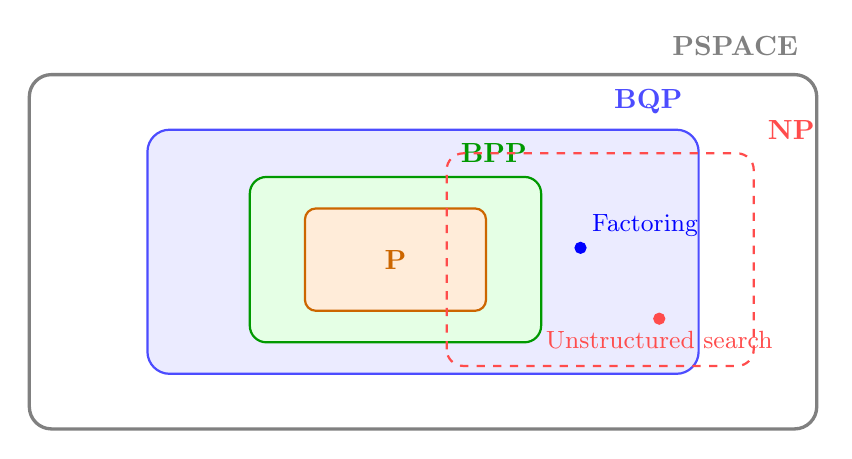
\begin{tikzpicture}[scale=1.0]
    % PSPACE outer box
    \draw[rounded corners=8pt, very thick, gray]
      (-5.0,-2.0) rectangle (5.0,2.5)
      node[above left=4pt] {\textbf{PSPACE}};
    % BQP ellipse
    \draw[rounded corners=8pt, thick, blue!70, fill=blue!8]
      (-3.5,-1.3) rectangle (3.5,1.8)
      node[above left=3pt, blue!70] {\textbf{BQP}};
    % BPP inner ellipse
    \draw[rounded corners=6pt, thick, green!60!black, fill=green!10]
      (-2.2,-0.9) rectangle (1.5,1.2)
      node[above left=2pt, green!60!black] {\textbf{BPP}};
    % P
    \draw[rounded corners=4pt, thick, orange!80!black, fill=orange!15]
      (-1.5,-0.5) rectangle (0.8,0.8);
    \node[orange!80!black] at (-0.35, 0.15) {\textbf{P}};
    % NP - overlapping with BQP but not subset
    \draw[rounded corners=6pt, thick, red!70, dashed]
      (0.3,-1.2) rectangle (4.2,1.5)
      node[above right=2pt, red!70] {\textbf{NP}};
    % Factoring dot
    \filldraw[blue] (2.0,0.3) circle (2pt)
      node[above right=1pt]{\small Factoring};
    % Search dot (Grover)
    \filldraw[red!70] (3,-0.6) circle (2pt)
      node[below=1pt]{\small Unstructured search};
  \end{tikzpicture}
  \caption{Believed relationships between complexity classes.
    BQP contains BPP (quantum solves everything classical probabilistic does) and is contained in PSPACE.
    BQP and NP are believed to be incomparable.
    Factoring sits in BQP but probably not in BPP.
    Unstructured search sits in both NP and BQP (with quadratic speedup), but Grover's speedup does not place NP $\subseteq$ BQP.
    Solid borders indicate certain inclusions; dashed borders indicate conjectured but unproven separation.
  }
\end{figure}

\section{Open Problems}

Quantum computing in 2025 stands at a pivotal moment.
The main open questions are both theoretical and engineering:

\begin{description}
  \item[Is $\mathrm{BQP}\neq\mathrm{BPP}$?]  We believe quantum computers are strictly more powerful than classical probabilistic ones, but this is not proved (it would imply $\mathrm{P}\neq \mathrm{PSPACE}$, an even harder open problem).

  \item[Post-quantum cryptography.] Even before fault-tolerant quantum computers exist, we must replace RSA and Diffie-Hellman with quantum-resistant schemes.
    NIST standardized several post-quantum algorithms in 2024 (CRYSTALS-Kyber for key encapsulation; \newline CRYSTALS-Dilithium and SPHINCS$^+$ for signatures).

  \item[NISQ applications.] Can near-term noisy quantum devices provide practical advantages for optimization, chemistry simulation, or machine learning before fault-tolerant hardware arrives?
    Variational algorithms (VQE, QAOA) are the main candidates, but clear practical advantage remains elusive.

  \item[Fault-tolerant hardware.] The main engineering challenge: reaching $\sim10^6$ physical qubits with error rates below threshold, with fast classical control electronics, and all operating coherently together.

  \item[Quantum networks.] Entanglement distribution over long distances (quantum repeaters) to enable global QKD and distributed quantum computing.
    The Chinese Micius satellite demonstrated satellite-based QKD over 1200 km in 2017.
\end{description}

The field is advancing rapidly.
Whether and when a practical, large-scale fault-tolerant quantum computer will exist remains unknown, but the theoretical framework developed in this course provides the foundation to understand both the possibilities and the fundamental limitations of quantum information processing.

\end{document}
